\chapter{Helixantenne}
Die zweite aufgebaute Antenne ist eine monofilare Helixantenne. Dieser Antennentyp ist gerichtet, was bedeutet, dass sie in eine bestimmte Richtung einen höheren Antennengewinn als in andere Richtungen hat. Sie ist eine der einfachsten Antennenarten um eine zirkulare Polarisation zu erzielen. Kombiniert mit ihrer hohen Bandbreite macht sie das zu einer attraktiven Option zum Nachbau und zur Verwendung in der Satellitenkommunikation. \cite{helixWebsite}

Für die in dieser Diplomarbeit konstruierte Helixantenne wurden die folgenden Vorgaben gewählt.

\begin{center}
	\begin{tabular}{|c|c|}
	\textbf{Parameter} & \textbf{Wert}\\
	Resonanzfrequenz & 433MHz\\
	Windungen & 6\\
	Abstand zwischen Windungen & $0,25\lambda$\\
	Polarisationsart & RHCP\\
	Betriebsmodus & Axial-Modus
\end{tabular}
\end{center}

Wobei $"$RHCP$"$ $"$Right Hand Circularily Polarized$"$ bedeutet. Für mehr Informationen zur zirkularen Polarisation wird auf den Abschnitt $"$\ref{subsec:pol} Polarisation$"$ verwiesen.

\section{Design}
Durch den Einsatz im Freien muss die Helixantenne einige Anforderungen erfüllen. Beispielsweise dürfen wichtige Strukturelemente unter UV-Einwirkung nicht brüchig werden, es darf sich durch Regen kein Wasser stauen und sie muss starkem Wind standhalten. 

Um die Helixantenne zu designen wurden Online-Rechner verwendet \cite{calculator_daycounter, calculator_jcoppens}.

\begin{center}
	\begin{tabular}{|c|c|}
	\textbf{Parameter} & \textbf{Wert} \\
	Wellenlänge &  692.8mm\\
	Durchmesser (intern) & 235.7mm\\
	Abstand zwischen den Windungen & 173.2mm\\
	Gesamthöhe & 1039.2mm\\
	minimaler Reflektor-Durchmesser & 429.5mm
\end{tabular}
\end{center}

Mithilfe dieser Werte wurde die erste Wendelantenne in Fusion 360 konstruiert. 

\begin{figure}[h!]
	\centering
	\includegraphics[width=5cm]{../ref/Erste Helixnäherung v0.png}
	\label{fig:ersteHelixnäherung}
	\caption{Das CAD-Modell für die Helixantenne mit den berechneten Werten}
\end{figure}

Diese wurde mithilfe von CENOS-Simulation-Suite für einen Frequenzbereich von [FREQUENZBEREICH] simuliert. Die Ergebnisse gaben Aufschluss über die Performance der Antenne in einer idealen Umgebung.

S11-Parameter
SWR
Abstrahlverhalten 2D
Abstrahlverhalten 3D

Es wurde der Schluss gezogen, dass die Resonanzfrequenz zu weit über dem gewünschten Wert von 433MHz liegt. Diese lässt sich durch Veränderung des Durchmessers der Spirale oder des Abstandes zwischen den Windungen verändern.

Durch das Abändern des Durchmessers konnte die gewünschte Resonanzfrequenz von 433MHz mit einem Helix-Durchmesser von 270mm erreicht werden. Der Reflektor wurde aus der Theorie mit ca. $\frac{3\lambda}{4}$ festgelegt \cite{Kraus-2002-AntennasB}, was einem Durchmesser von ungefähr 520mm entspricht.

Es ist wichtig anzumerken, dass der Steigungswinkel der Spirale hierbei ca. 11,5° beträgt. Dies bedeutet, dass die Steigung von dem relativ engen Idealbereich zwischen 12° und 14° abweicht.

\section{Realisierung}
Die Helixantenne benötigt zur Funktion nur zwei Bauteile: die Spirale und der Reflektor. Für die Simulation genügt dieses Modell, allerdings werden in der Realität Strukturelemente benötigt um diese zu befestigen.

\begin{figure}[H]
	\centering
	\includegraphics[width=10cm,angle=270]{../ref/Helixantenne-real.jpg}
	\caption{Reale Helixantenne}
	\label{fig:helix-real}
\end{figure}

\begin{tabular}{|c|c|c|c|c|}
	\hline
	Nr. & Typ & Maße & Besonderheiten & Menge \\
	\hline
	1 & PVC-Rohr & 50x3,7mm 1m & UV-stabilisiert & 4x \\
	\hline
	2 & Teflon-Rundlinge & \O 10mm 2m & Abstandhalter & 4x \\
	\hline
	3 & Rohrflansch (Antenne) & \O innen 51mm &  & 4x \\
	\hline
	4 & Rohrflansch (Struktur) & \O innen 45mm &  & 2x \\
	\hline
	5 & Aluminiumrohr & 18x2mm 5,2m & Spirale & 4x \\
	\hline
	6 & Runde Aluminiumplatte & \O 520x3mm & Reflektor & 4x \\
	\hline
\end{tabular}

Das schwarze PVC-Stützrohr ist UV-stabilisiert. Wäre der Kunststoff nicht gegen UV-Strahlung geschützt, so würde dieser nach einer Zeit spröde und strukturell unzuverlässig.

In das PVC-Rohr wurden Löcher mit einem Abstand von 86,6mm und einem Durchmesser von 11mm gebohrt. Diese schaffen genug Platz für die Seitenelemente welche einen Durchmesser von 10mm aufweisen. Um das Rohr mithilfe des Rohrflansches an der Reflektorplatte zu montieren wurden zwei Löcher mit M10-Gewinde gebohrt. Für die Konstruktionszeichnung wird auf Kapitel \ref{chap:Anhang} verwiesen.

Das gewählte Material ist PTFE, da es eine sehr niedrige elektrische Permittivität besitzt. Das ist wichtig, da die Spirale, welche die Resonanzfrequenz der Helixantenne bestimmt, so gut wie möglich von kapazitiven Einflüssen geschützt sein sollte. Das $\epsilon\textsubscript{r}$ von PTFE ist rund 2,2, während das von Luft ca. 1 ist \cite{lipinski_polytetrafluorethylen_nodate,noauthor_dielektrizitatskonstante_nodate}. Teflon ist zwar ein relativ weicher Kunststoff, allerdings ist Aluminium ein sehr leichtes Metall, welches durch die Teflonstäbe sicher gestützt werden kann. Da PTFE UV-beständig und ein allgemein widerstandsfähiger Kunststoff ist, eignet dieser sich bestens für den Einsatz im Freien. Für den Konstruktionsplan des Abstandhalters wird auf Kapitel \ref{chap:Anhang} verwiesen.

\begin{figure}[h!]
	\centering
	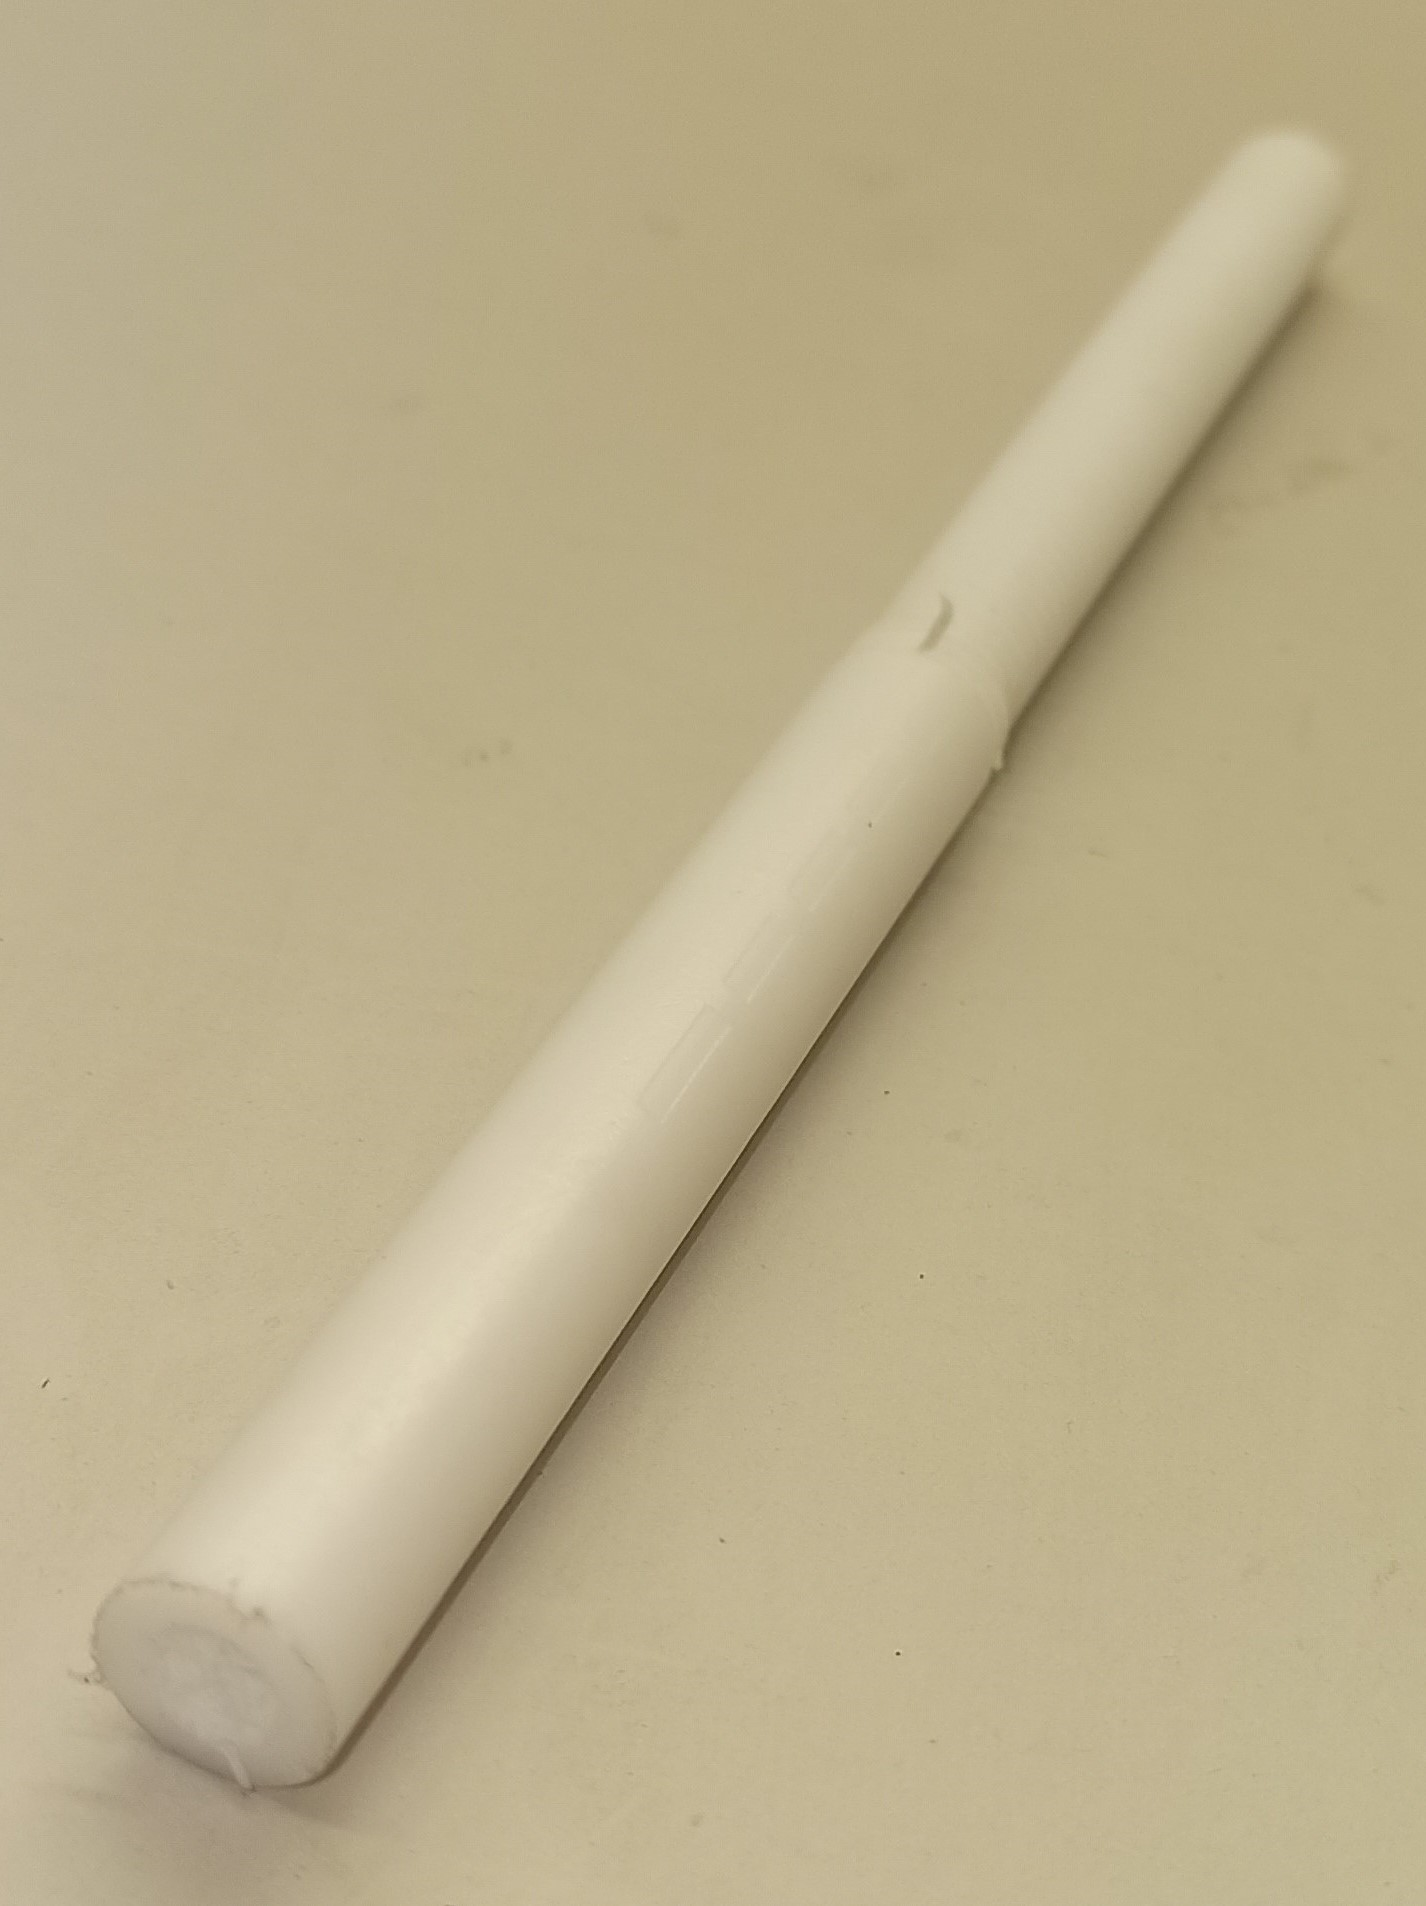
\includegraphics[width=5cm]{../ref/Abstandhalter-real.jpg}
	\caption{Realer Abstandhalter}
	\label{fig:Abstandhalter-real}
\end{figure}

An der Zeichnung sowie an dem realen Bauteil lässt sich erkennen, dass das Außengewinde ungefähr bis zur Hälfte der Teflonstange geschnitten ist. Der Stab wird mit dem Gewinde zuerst in die Löcher des PVC-Rohres gesteckt, damit dieser von vorne und hinten mit M10-Kunststoffmuttern an das Rohr geschraubt werden kann.

In die andere Seite des Abstandhalters wird ein Loch mit einem Durchmesser von 5mm für ein M6-Gewinde gebohrt. Mithilfe der entsprechenden Schrauben werden UV-stabilisierte Rohrschellen an dem Seitenelement montiert. Diese tolerieren Rohrdurchmesser von bis zu 18mm. Durch die Verwendung von Rohrschellen vereinfacht sich die Montage der Spirale auf ein einfaches Einschnappen des Rohres.

\begin{figure}[H]
	\begin{minipage}[b]{.4\linewidth} % [b] => Ausrichtung an \caption
		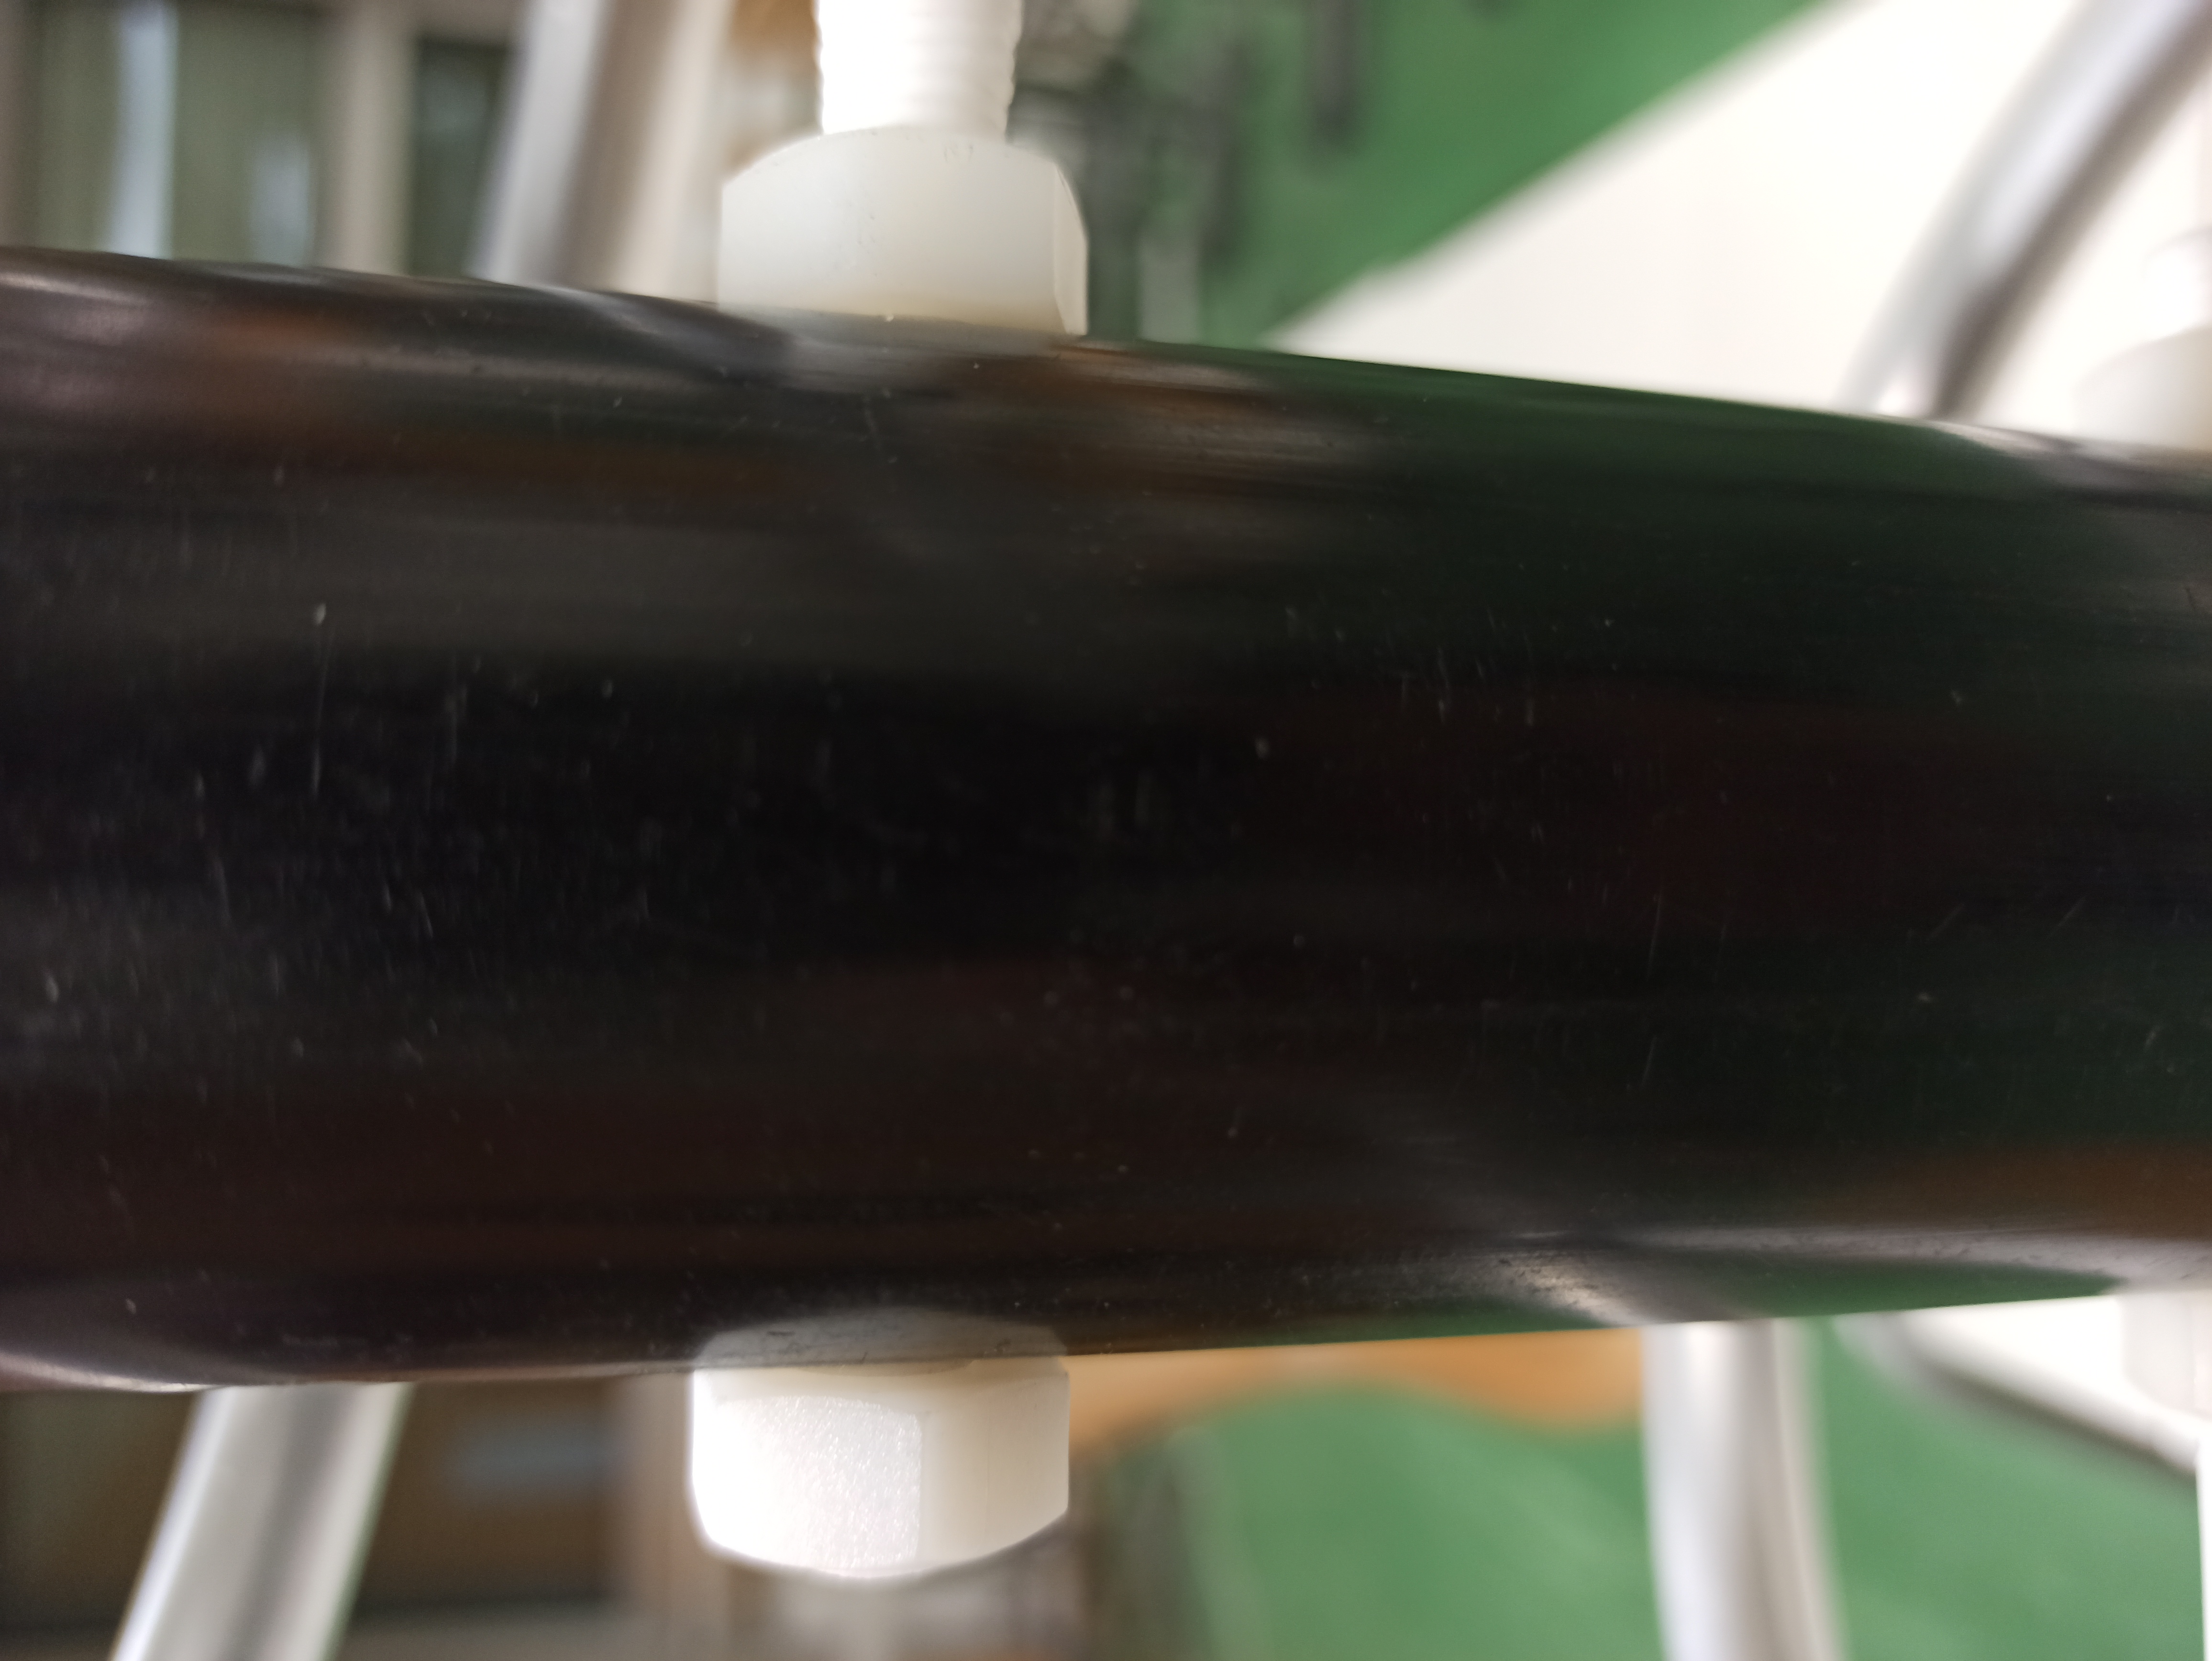
\includegraphics[width=7cm, angle=270]{../ref/Befestigung-Querelement.jpg}
		\label{fig:Abstandhalter-Befestigung}
	\end{minipage}
	\hspace{.1\linewidth}% Abstand zwischen Bilder
	\begin{minipage}[b]{.4\linewidth} % [b] => Ausrichtung an \caption
		\includegraphics[width=7cm, angle=270]{../ref/Rohrklemme-an-Spirale.jpg}
		\label{fig:Seitenelement-an-Spirale}
	\end{minipage}
	\caption{Links: Befestigung des Abstandhalters am Rohr. Rechts: Eingeschnappter Abstandhalter an der Spirale}
\end{figure}

Der Rohrflansch bildet das Bindeelement zwischen dem PVC-Rohr und der Reflektorplatte. Dieser hat einen Innendurchmesser von 51mm, und eine Wandstärke von 4mm. Dadurch wird genug Toleranz geboten damit das PVC-Rohr sicher verschraubt werden kann. 

Der Rohrflansch besteht aus einem Rohr, in welches zwei durchgehende Löcher mit einem Durchmesser von 11mm gebohrt wurden, und einer Platte in die ebenfalls zwei Löcher mit einem Durchmesser von 13,5mm gebohrt wurden. Die Platte und das Rohr werden aneinander geschweißt. Das resultierende Bauteil bildet das Bindeglied zwischen Reflektor und PVC-Rohr.

%NOCH UMZUFORMULIEREN
Für den Reflektor wurde eine runde Aluminiumplatte gewählt. Für die reale Konstruktion wurden Löcher in den äußeren Rand der Platte gelasert, um den Luftwiderstand zu reduzieren. Um eventuelle Störungen durch spezifische Maße wie beispielsweise $\frac{\lambda}{4}$ zu vermeiden, wurden die Löcher um einiges kleiner als $\frac{\lambda}{4}$ gewählt.

\begin{figure}[H]
	\begin{minipage}[b]{.4\linewidth} % [b] => Ausrichtung an \caption
		\includegraphics[width=7cm,angle=270]{../ref/Rohrflansch-Antenne.jpg}
		\caption{Befestigung des Rohrflansches}
		\label{fig:Rohrflansch-Antenne-Verbindung}
	\end{minipage}
	\hspace{.1\linewidth}% Abstand zwischen Bilder
	\begin{minipage}[b]{.4\linewidth} % [b] => Ausrichtung an \caption
		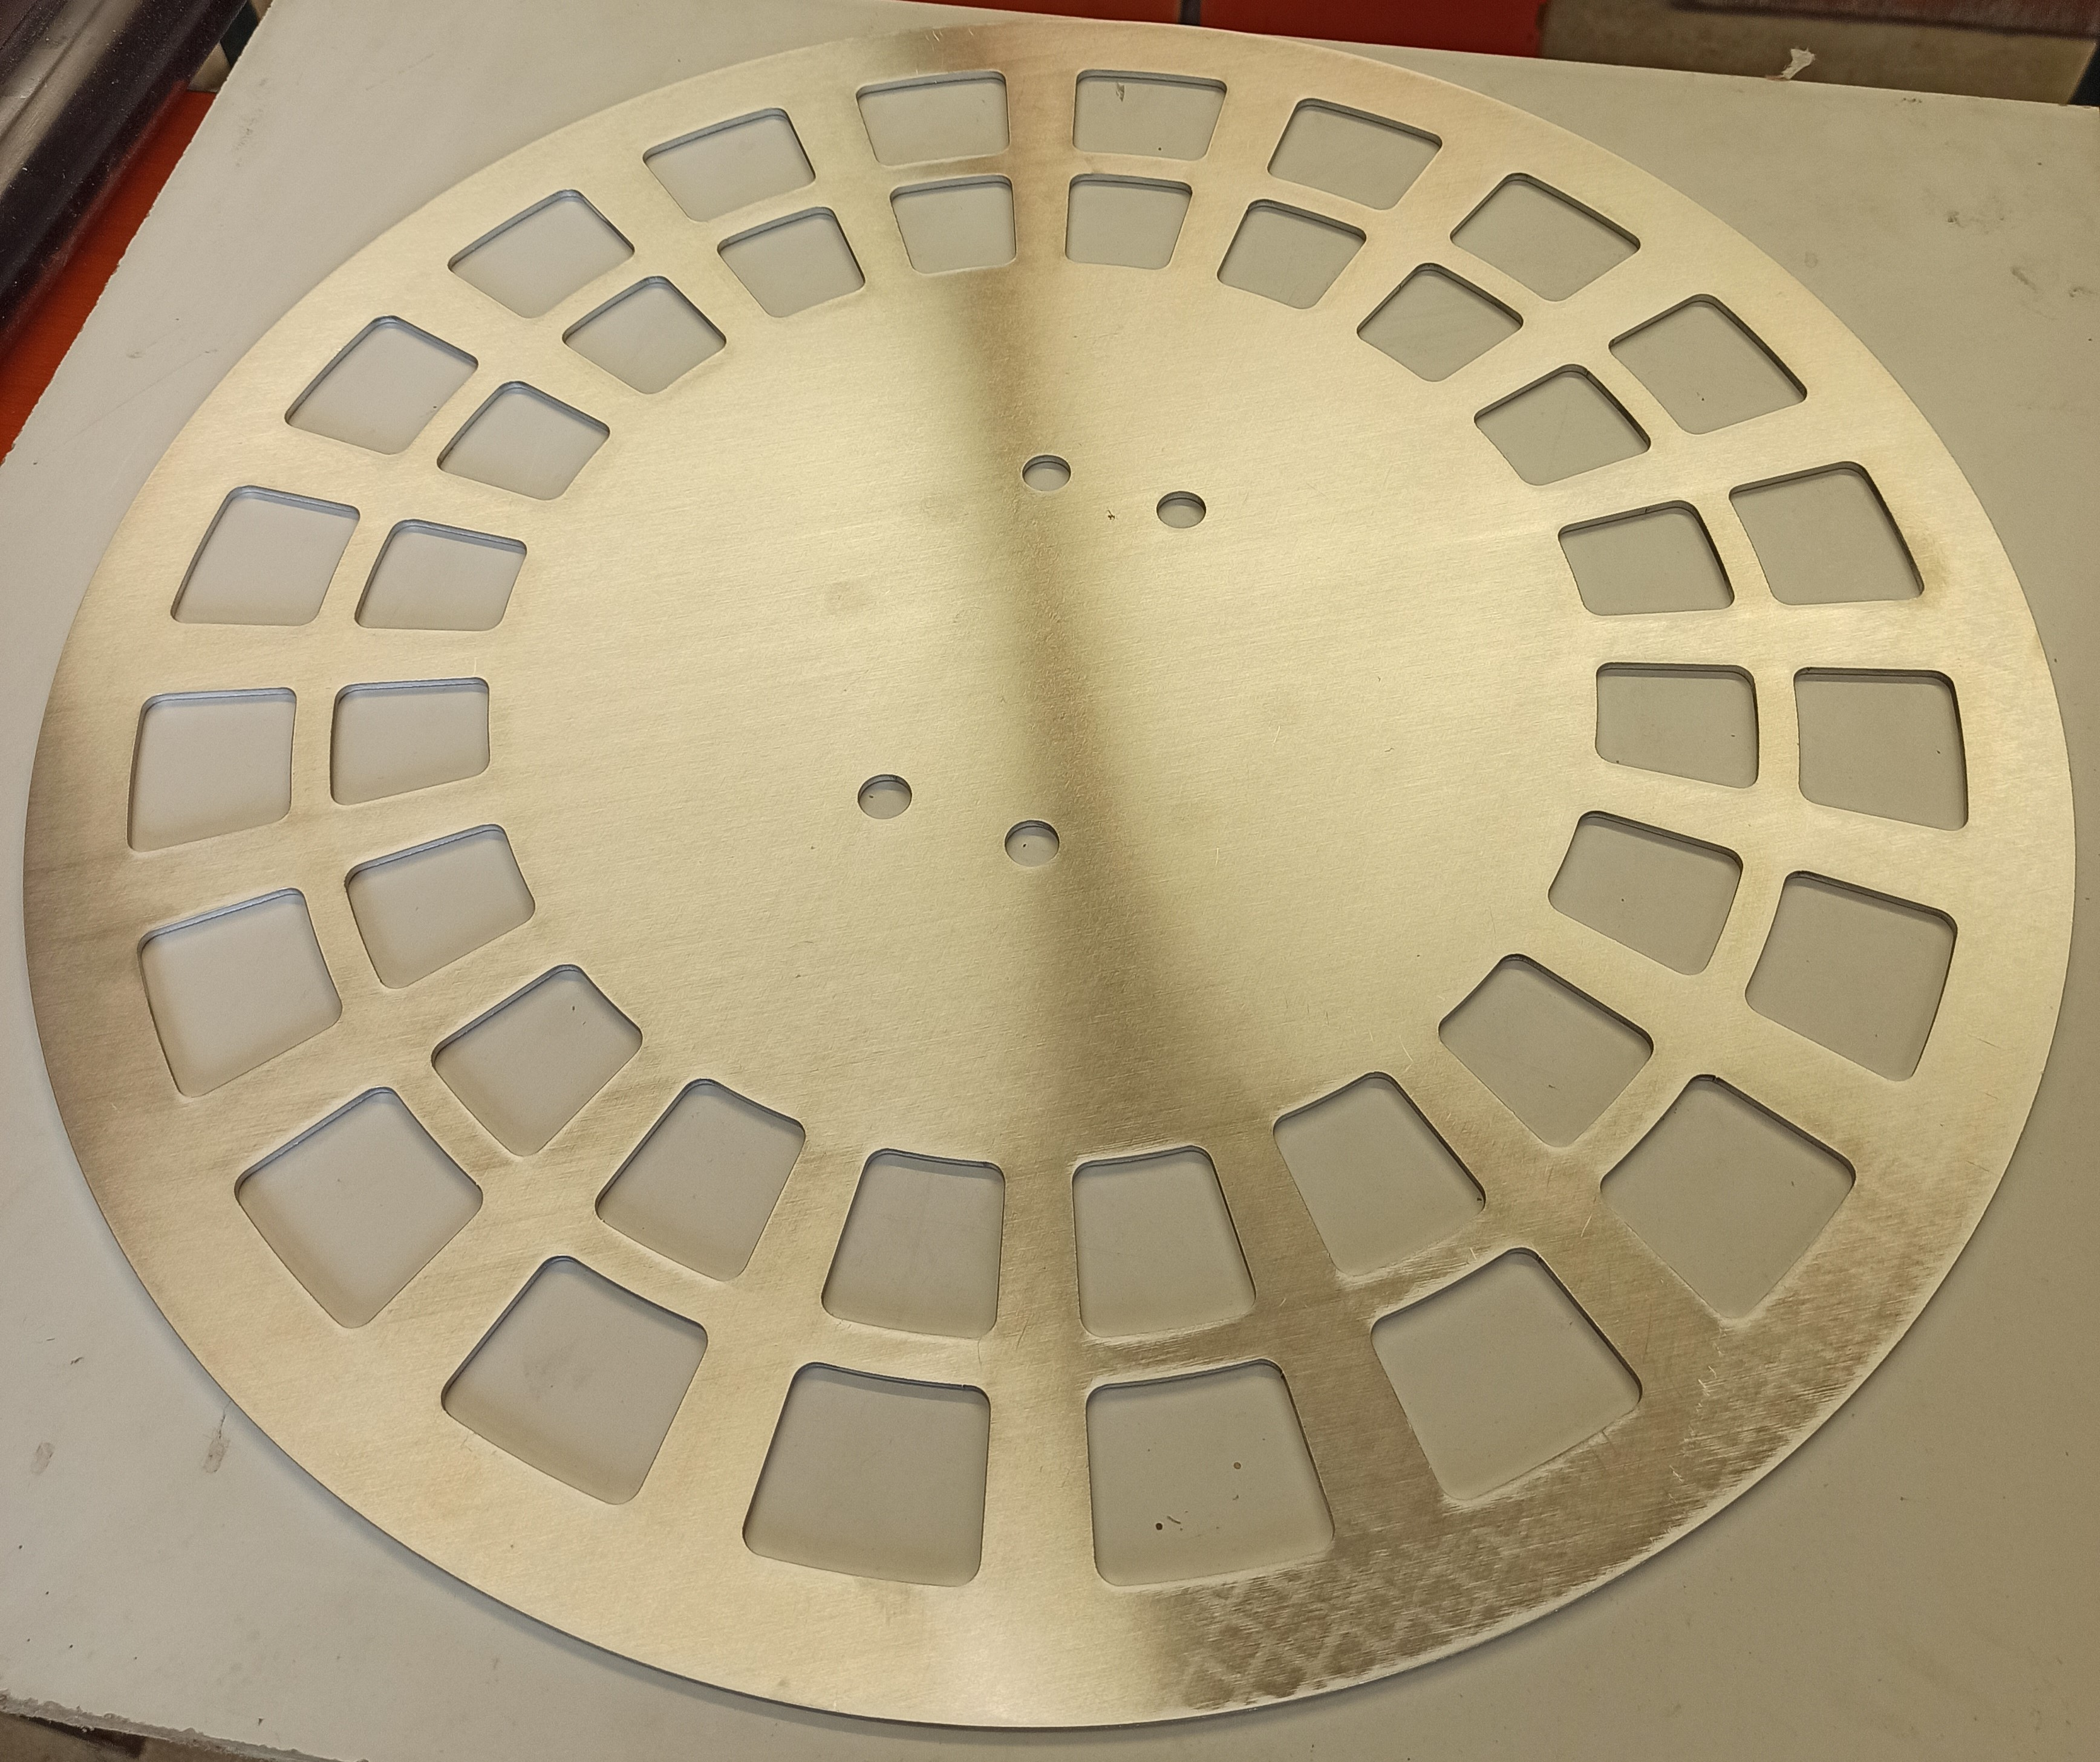
\includegraphics[width=7cm]{../ref/Reflektor.jpg}
		\caption{Reflektor der Wendelantenne}
		\label{fig:Reflektor}
	\end{minipage}
\end{figure}

In der Mitte des Reflektors werden vier Löcher mit einem Durchmesser von 13,5mm gebohrt an denen der Rohrflansch befestigt wird. 

Die Helix wurde real ebenso gebogen wie in der Simulation. Es wurde ein Aluminiumrohr verwendet, welches zu einer Spirale gebogen wurde, welche einen Durchmesser von 270mm, eine Höhe von ca. 1039,2mm und konsequent eine Steigung von 11,5° beziehungsweise einen Abstand zwischen den Windungen von 173,2mm ($\frac{\lambda}{4}$) hat.

\begin{figure}[H]
	\centering
	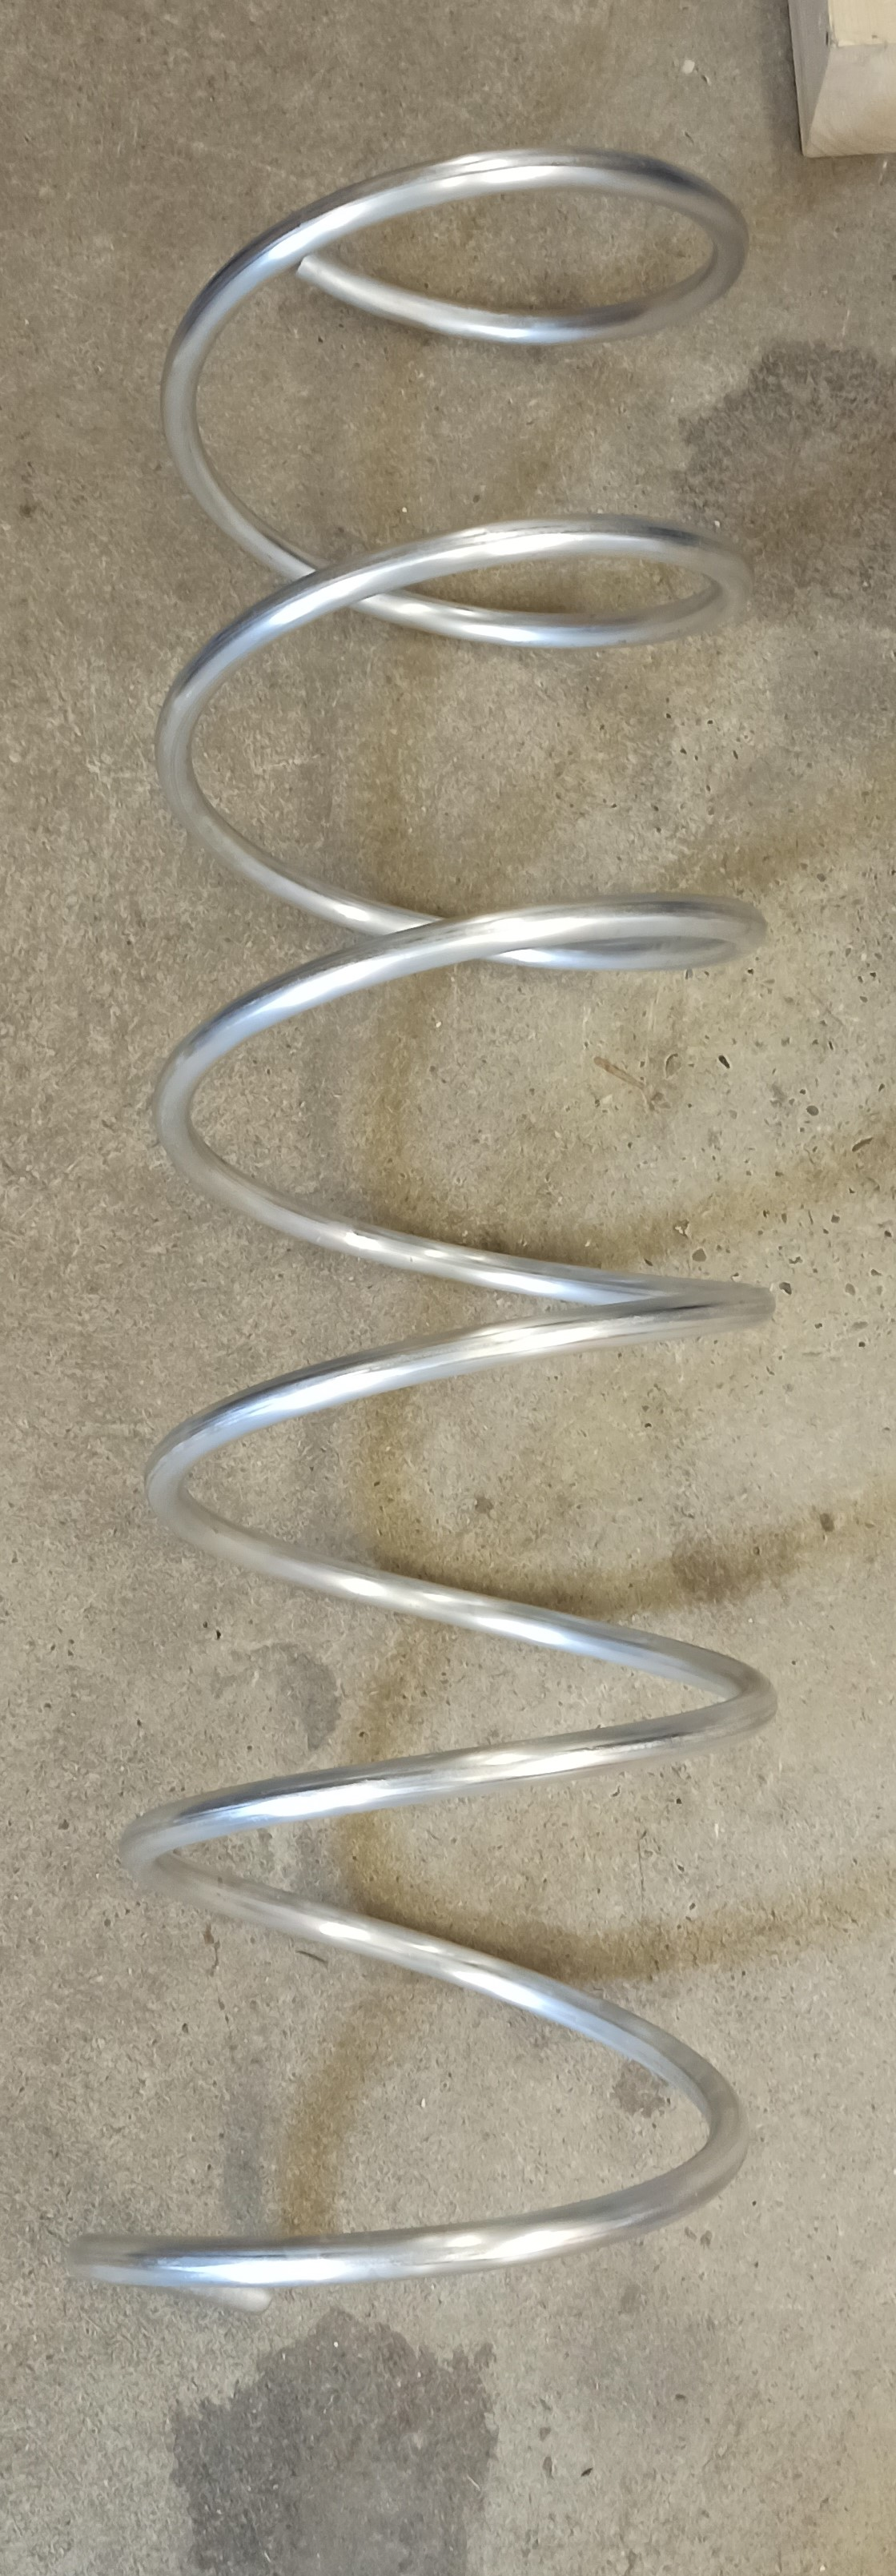
\includegraphics[width=5cm,angle=90]{../ref/Spirale.jpg}
	\caption{Das charakteristische Merkmal der Wendelantenne: die Spirale}
	\label{fig:Spirale}
\end{figure}

Um die Helixantenne wasserdicht zu machen wurden kurz abgeschnittene Aluminium-Rundlinge auf die Öffnungen der Spirale geschweißt. Am unteren Ende der Helix, an der der Innenleiter des Koaxialkabels befestigt wird, wurde ein Gewinde in den Aluminiumrundling geschnitten.

\begin{figure}[h!]
	\begin{minipage}[b]{.4\linewidth} % [b] => Ausrichtung an \caption
		\includegraphics[width=\linewidth]{../ref/Deckel-oben.jpg}
		\label{fig:Deckel-Helix-Oben}
	\end{minipage}
	\hspace{.1\linewidth}% Abstand zwischen Bilder
	\begin{minipage}[b]{.4\linewidth} % [b] => Ausrichtung an \caption
		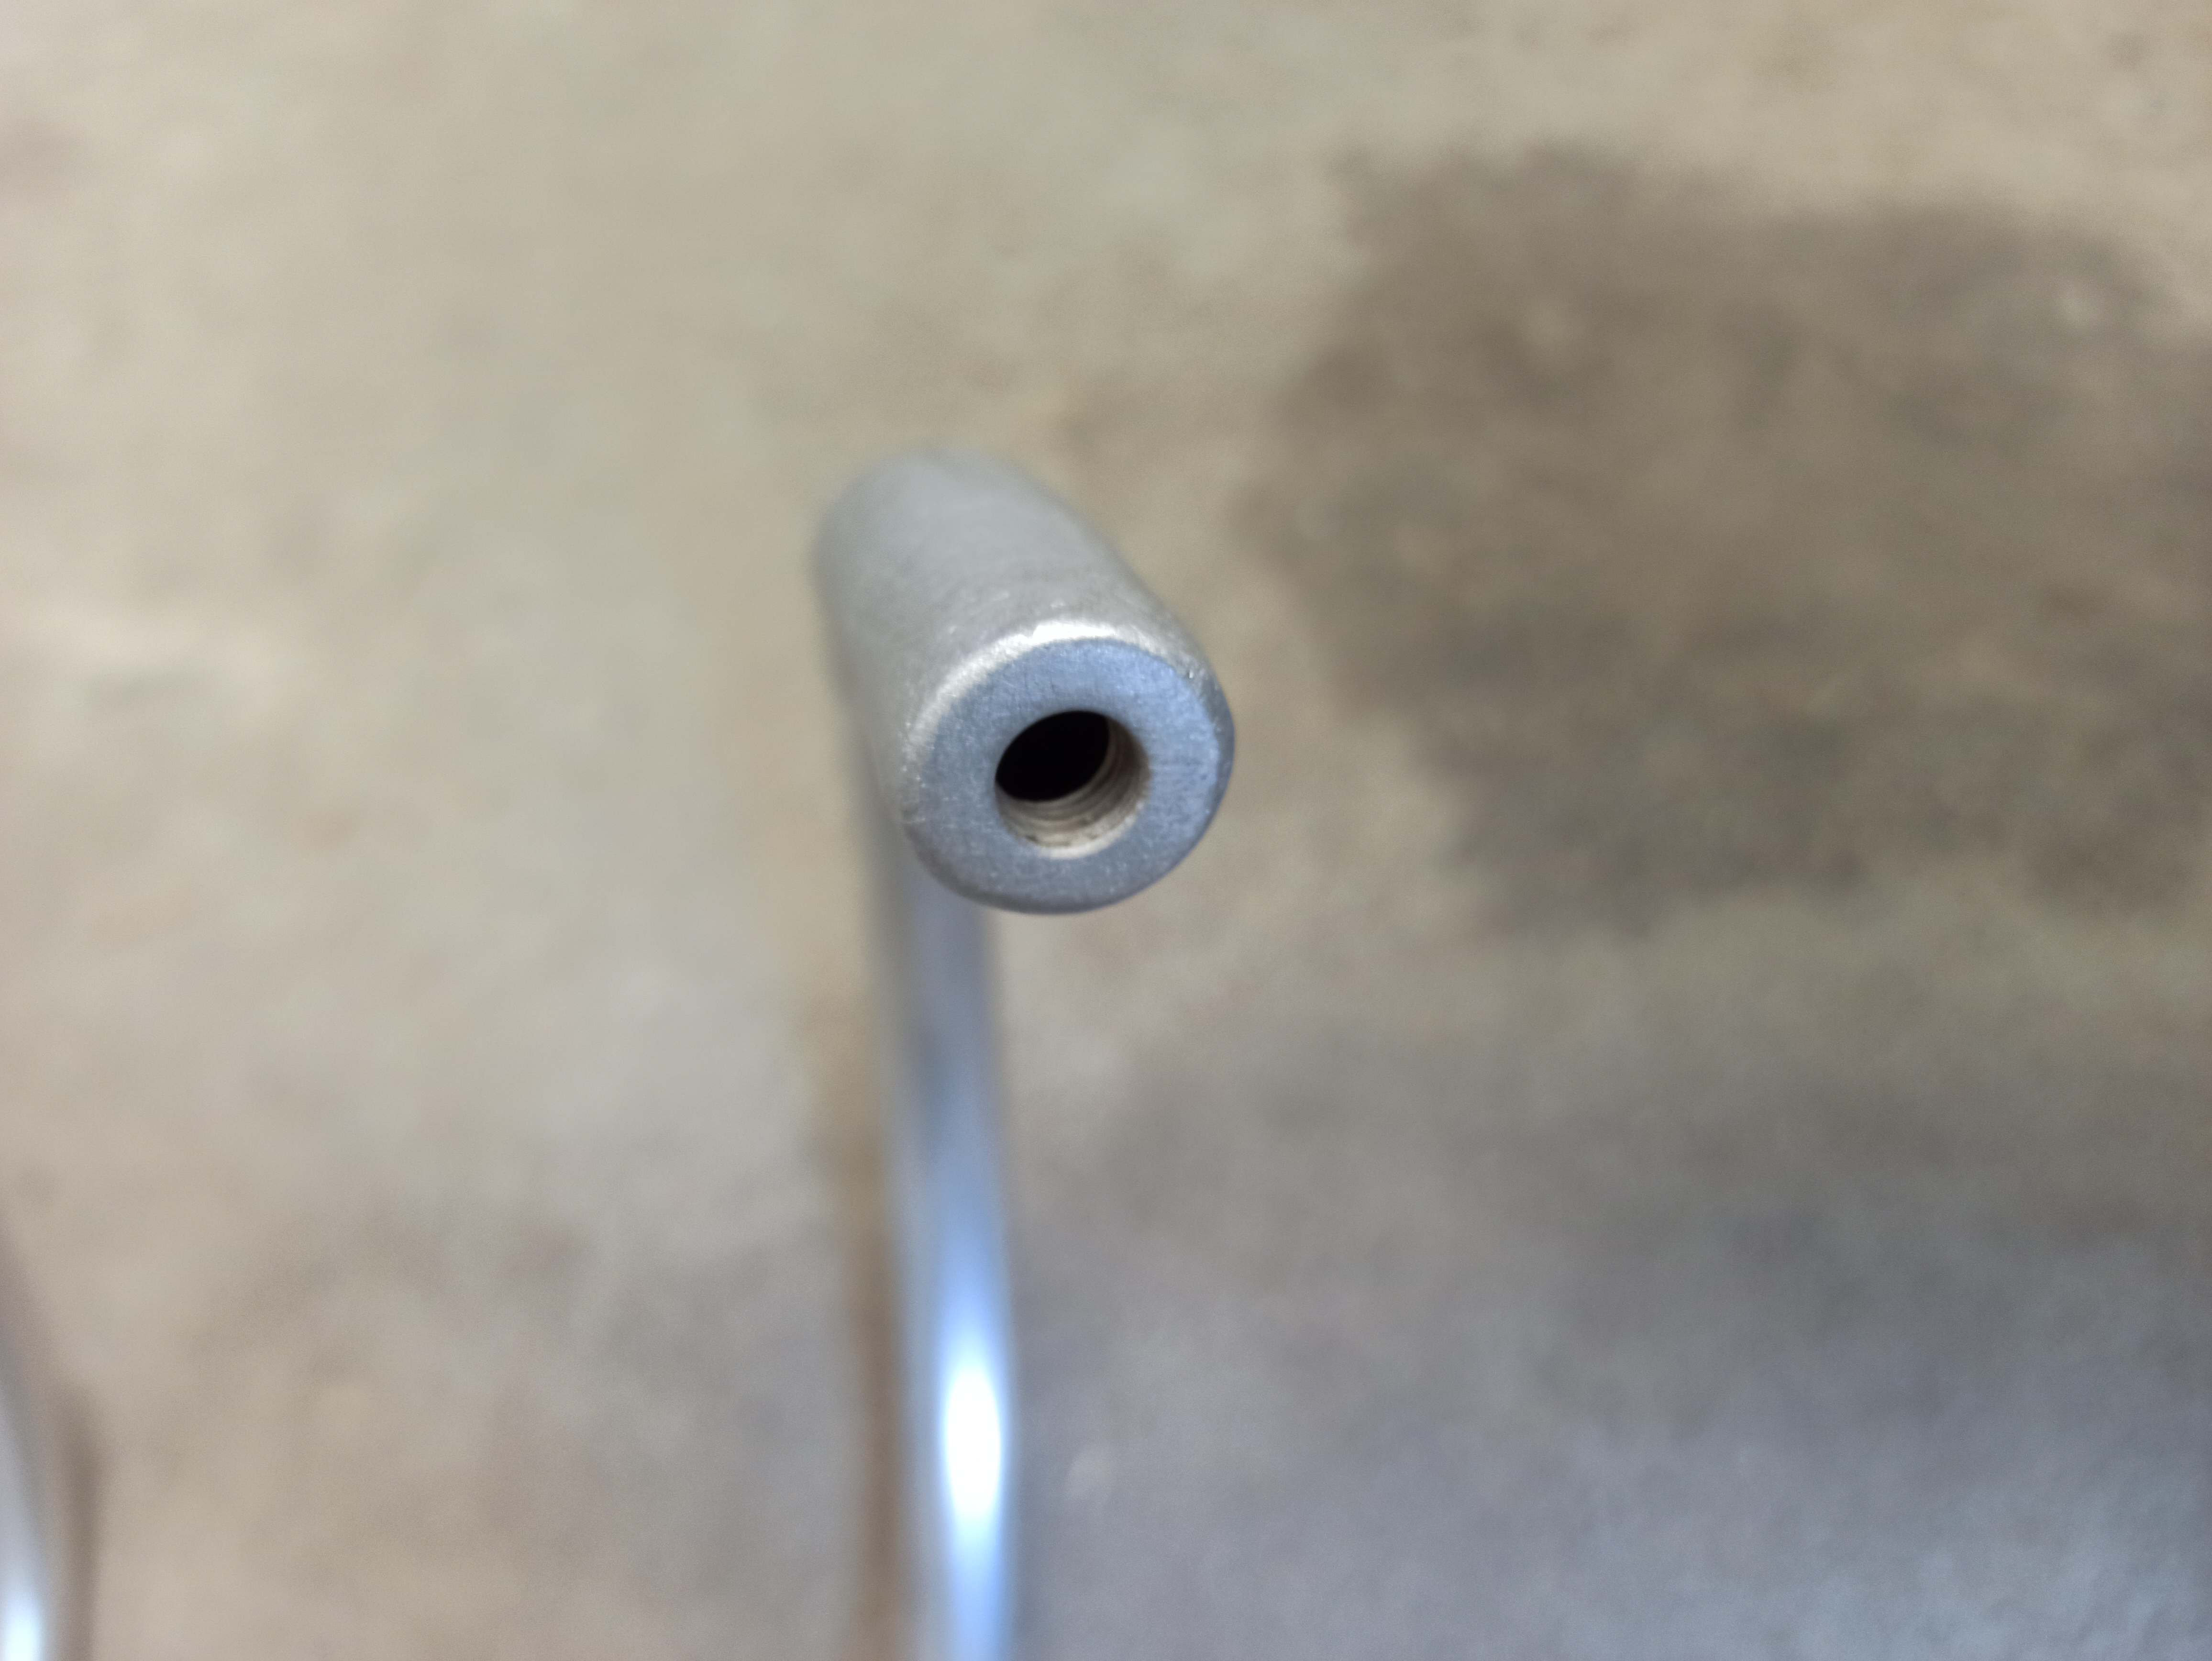
\includegraphics[width=\linewidth]{../ref/Anschluss-unten.jpg}
		\label{fig:Deckel-Helix-Unten}
	\end{minipage}
	\caption{Links: Zugeschweißtes oberes Ende der Helix. Rechts: Gewinde am unteren Ende der Helix zur Anbringung des Innenleiters}
\end{figure}

Mithilfe dieses Gewindes kann ein Kabel durch eine Schraube montiert, und am Innenleiter der BNC-Buchse angelötet werden.

Um die PVC-Rohre vor Wasser zu schützen wurden Abdeckungen 3D-gedruckt. Durch die Verwendung eines speziellen Filaments vom Typ DuraPro ASA, ist das Resultat eine UV-resistente Rohrabdeckung. Durch diese Eigenschaft eignet sich dieses Filament exzellent für den Einsatz im Freien.

\begin{figure}[h!]
	\centering
	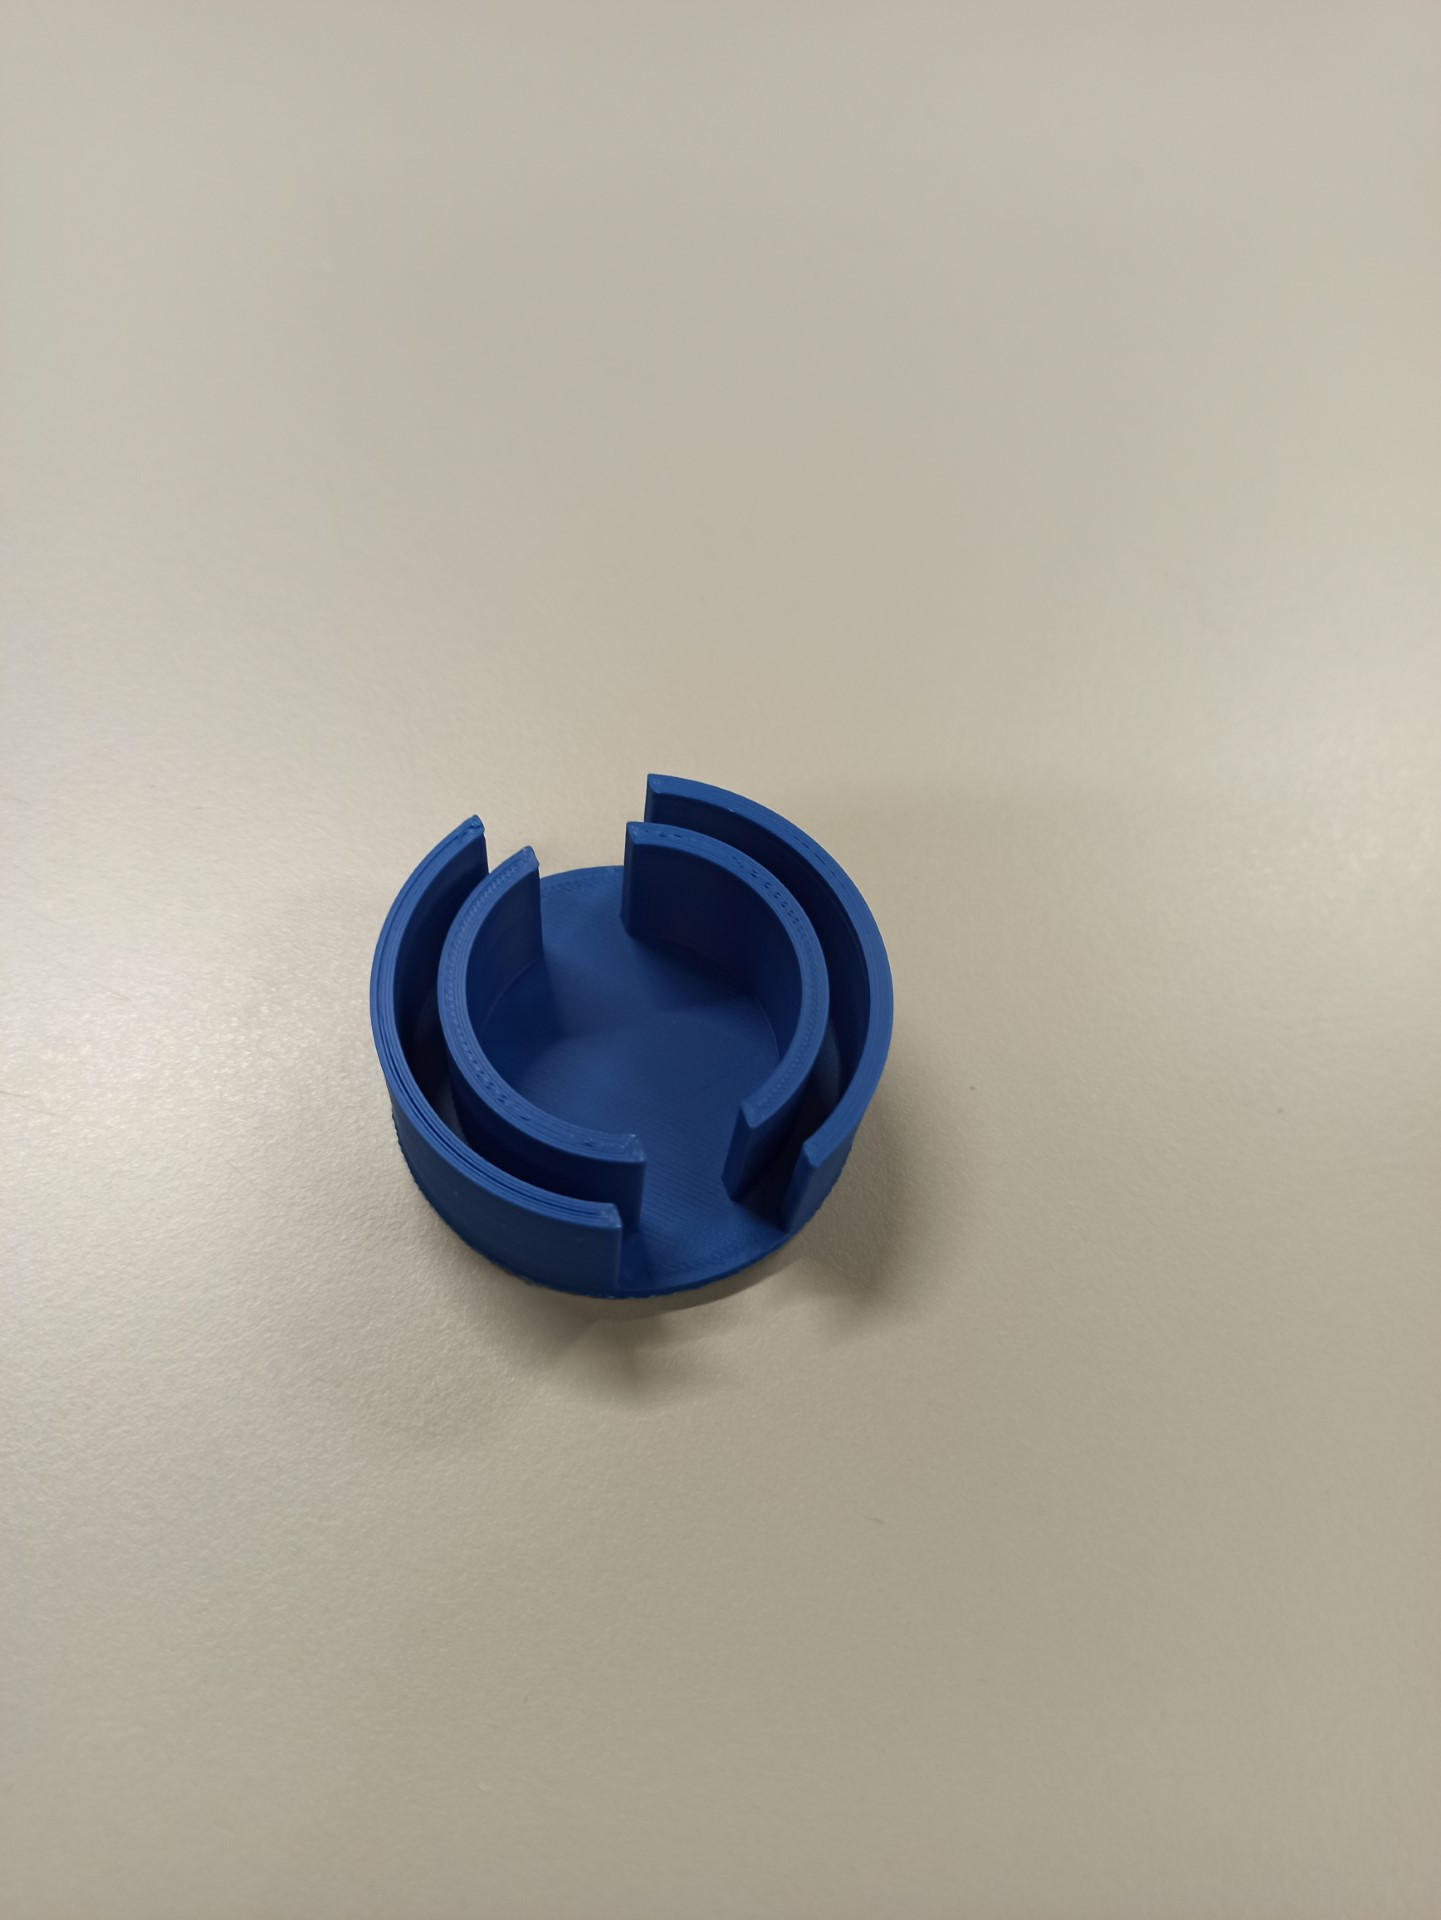
\includegraphics[width=5cm]{../ref/Abdeckung-PVC-Rohr.jpg}
	\caption{Die Abdeckung des PVC-Rohres}
	\label{fig:PVC-Rohr-Abdeckung}
\end{figure}

Die BNC-Buchse befindet sich direkt unter dem Ende der Spirale. Der Innenleiter wird, wie bereits erwähnt, an der Helix befestigt. Der Außenleiter wird mit dem Reflektor verschraubt.

\begin{figure}[h!]
	\begin{minipage}[b]{.4\linewidth} % [b] => Ausrichtung an \caption
		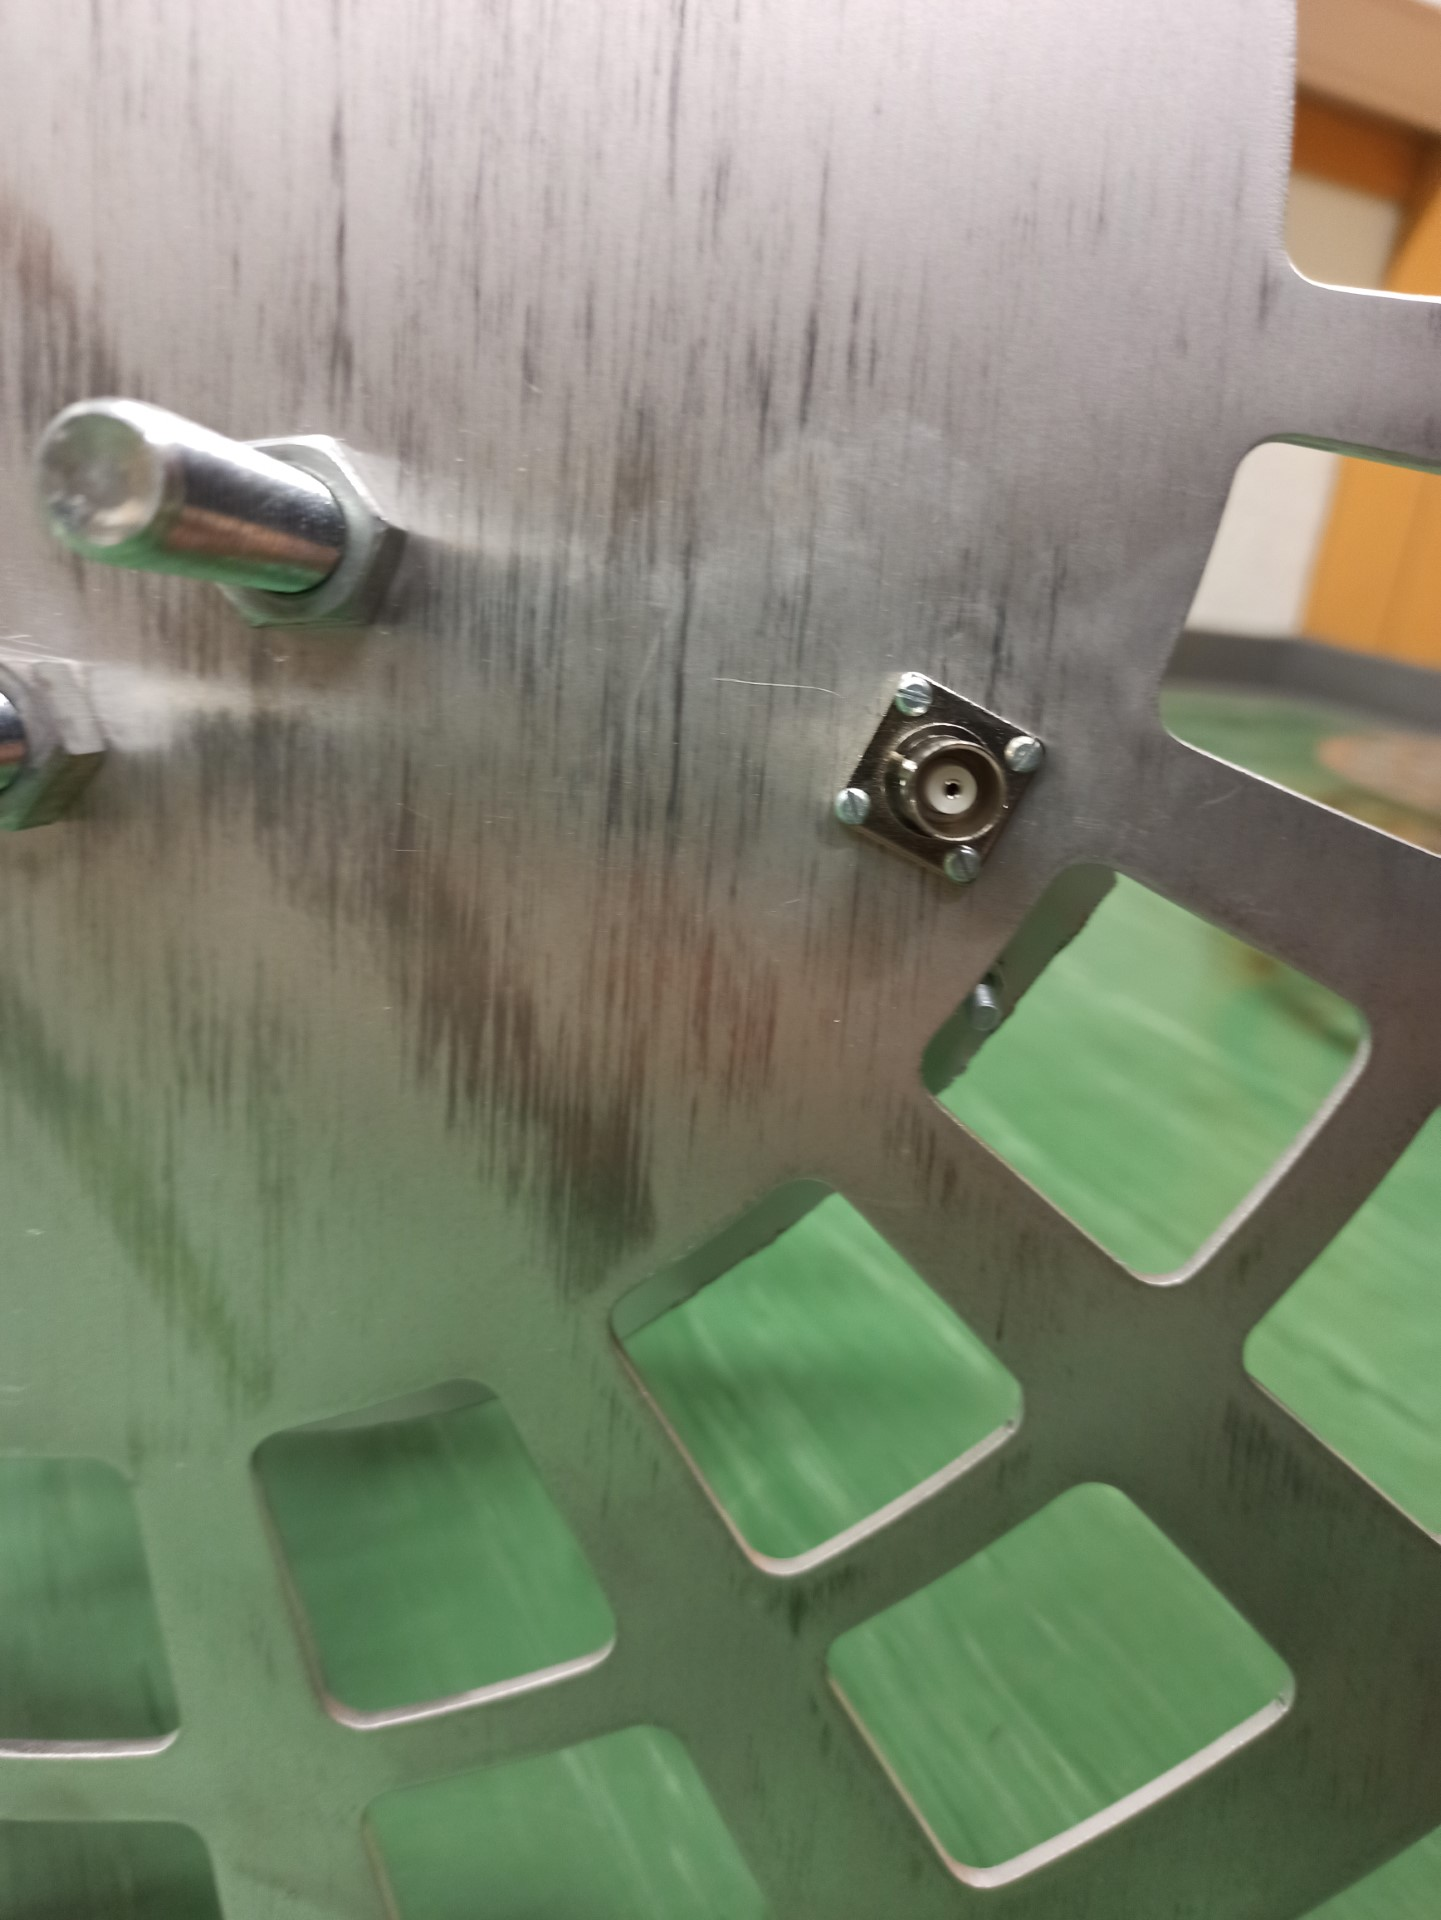
\includegraphics{../ref/BNC-Buchse.jpg}
		\label{fig:BNC-Buchse}
	\end{minipage}
	\hspace{.1\linewidth}% Abstand zwischen Bilder
	\begin{minipage}[b]{.4\linewidth} % [b] => Ausrichtung an \caption
		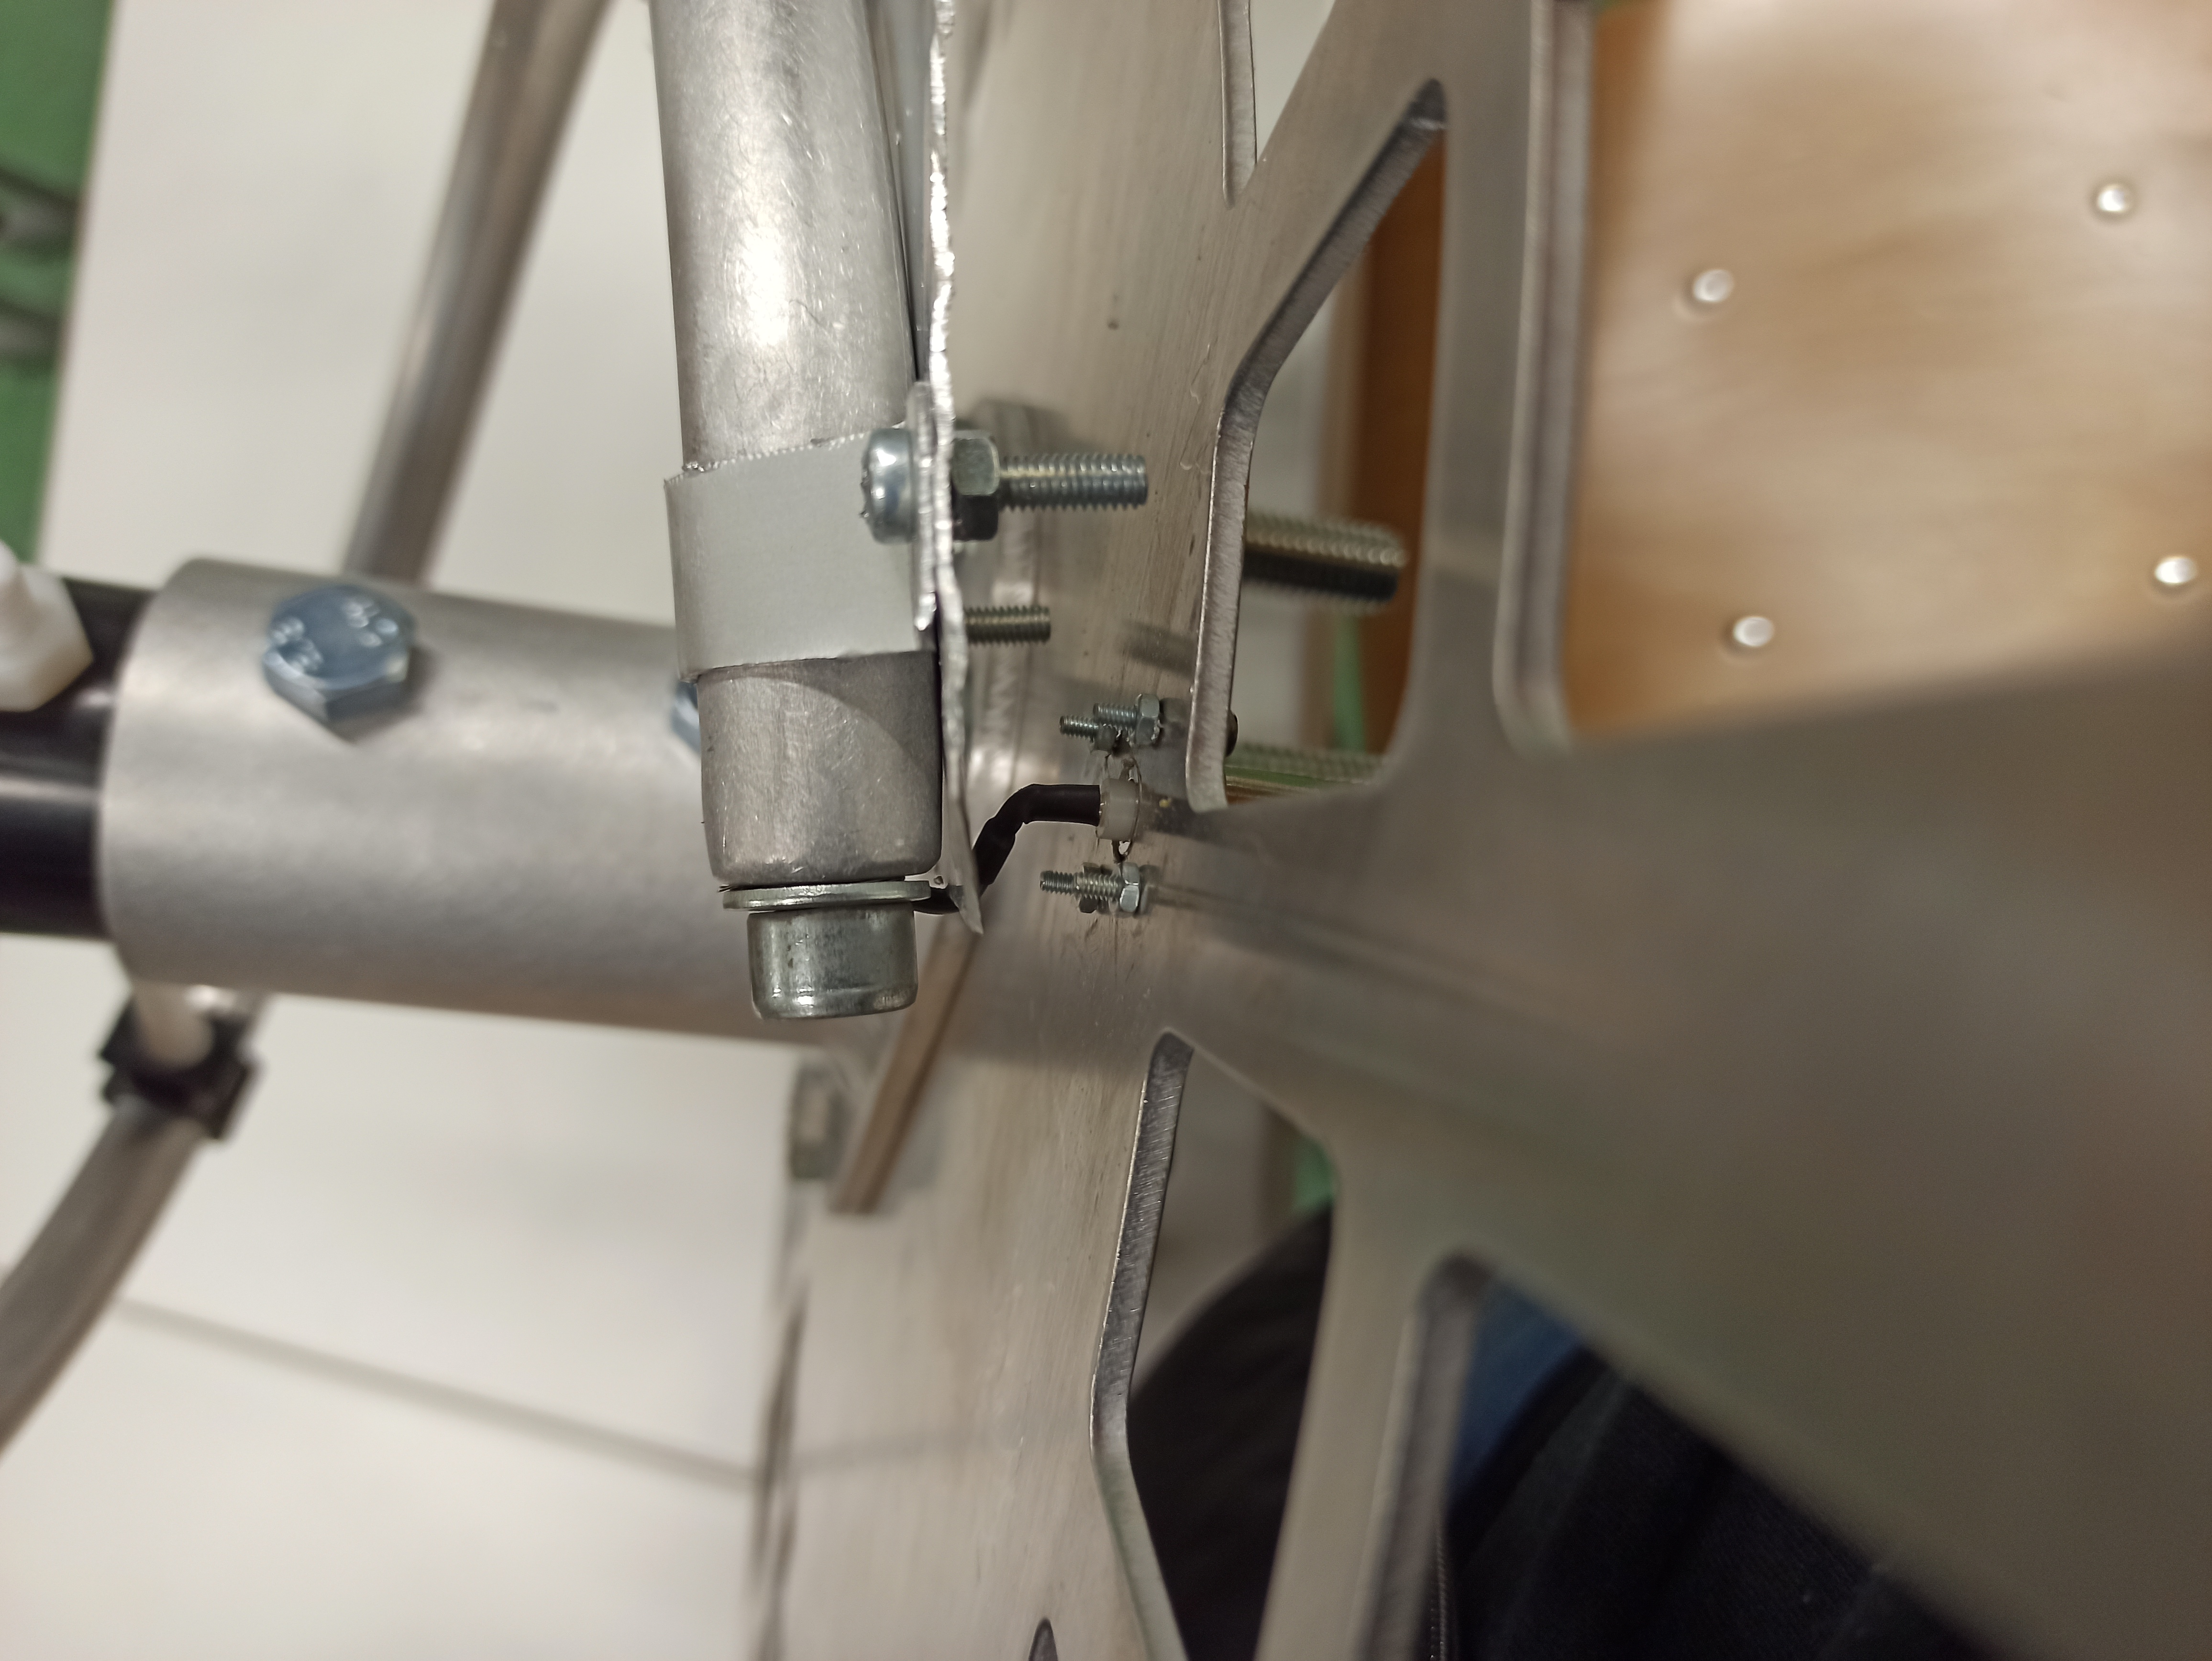
\includegraphics[angle=270]{../ref/Befestigung-Innenleiter.jpg}
		\label{fig:Innenleiter-Befestigung}
	\end{minipage}
	\caption{Koaxialkabel-Anschluss}
\end{figure}



\section{Anpassung}
Um eine einzelne Helixantenne anzupassen gibt es verschiedene Möglichkeiten. Eine weit verbreitete Option ist es, einen entsprechend dimensionierten Blechstreifen mit einer Länge von $\frac{\lambda}{4}$ entlang des unteren Endes der Helix zu montieren. Dieser agiert als Resonanztransformator und soll die Impedanz der Antenne auf einen Wert von 50$\Omega$ senken \cite{kgwadi_parametric_2014}.

\begin{figure}[H]
	\centering
	\includegraphics[width=7cm]{../ref/Anpassstreifen.jpg}
	\caption{Der realisierte Blechstreifen für die Impedanzanpassung}
	\label{fig:matching-strip}
\end{figure}

Die Breite des Blechstreifens wurde empirisch ermittelt und wurde mit 6cm festgelegt. Um den S11-Parameter auf einen akzeptablen Wert zu bringen, wird der Abstand zwischen Reflektor und Spirale verringert. Dadurch beeinflussen sich der Blechstreifen und die auf Masse liegende Reflektorplatte auf eine Weise, die der Performance der Antenne zugutekommt.

\section{Tests}
Tests im Freien, Messungen an Satelliten

\section{Erweiterung der Helixantenne als Array}
Nun wird die Helixantenne durch drei weitere identische Helixantennen erweitert, welche zusammen ein Array bilden. Hierbei ist der Abstand zwischen den einzelnen Antennen von Relevanz um den Gesamtgewinn zu maximieren.
Der Antennengewinn eines Antennenarrays bestehend aus vier identischen Helixantennen liegt in der Theorie bei dem vierfachen Antennengewinn einer einzelnen Wendelantenne, bzw. einer Helixantenne mit der vierfachen Windungszahl, also $4*6=24$. QUELLE

Hierfür muss ein Gerüst designt und aufgebaut werden, welches vier solcher Antennen halten kann, sowie die neu entstehende Impedanz der Zusammenschaltung dieser Antenne angepasst werden. Anschließend müssen Tests durchgeführt werden, die den verbesserten Antennengewinn der Antenne belegen.

\subsection{Gerüst}

\begin{tabular}{|c|c|c|c|}
	\hline
	Nr. & Typ & Maße & Menge \\
	\hline
	1 & Aluminiumrohr & \O42x2,5mm 0,77m & 1x \\
	\hline
	2 & Aluminium-Vierkantrohr & 60x100x3mm 0,9m & 2x \\
	\hline
\end{tabular}

Als Gerüst wurde die Form eines $"$H$"$ gewählt. Da der Schwerpunkt des Gerüsts im Mittelpunkt liegt, wird das vom Rotor benötigte Moment minimiert. 

%Gegenüberstellung zu realem Gerüst
\begin{figure}[h!]
	\centering
	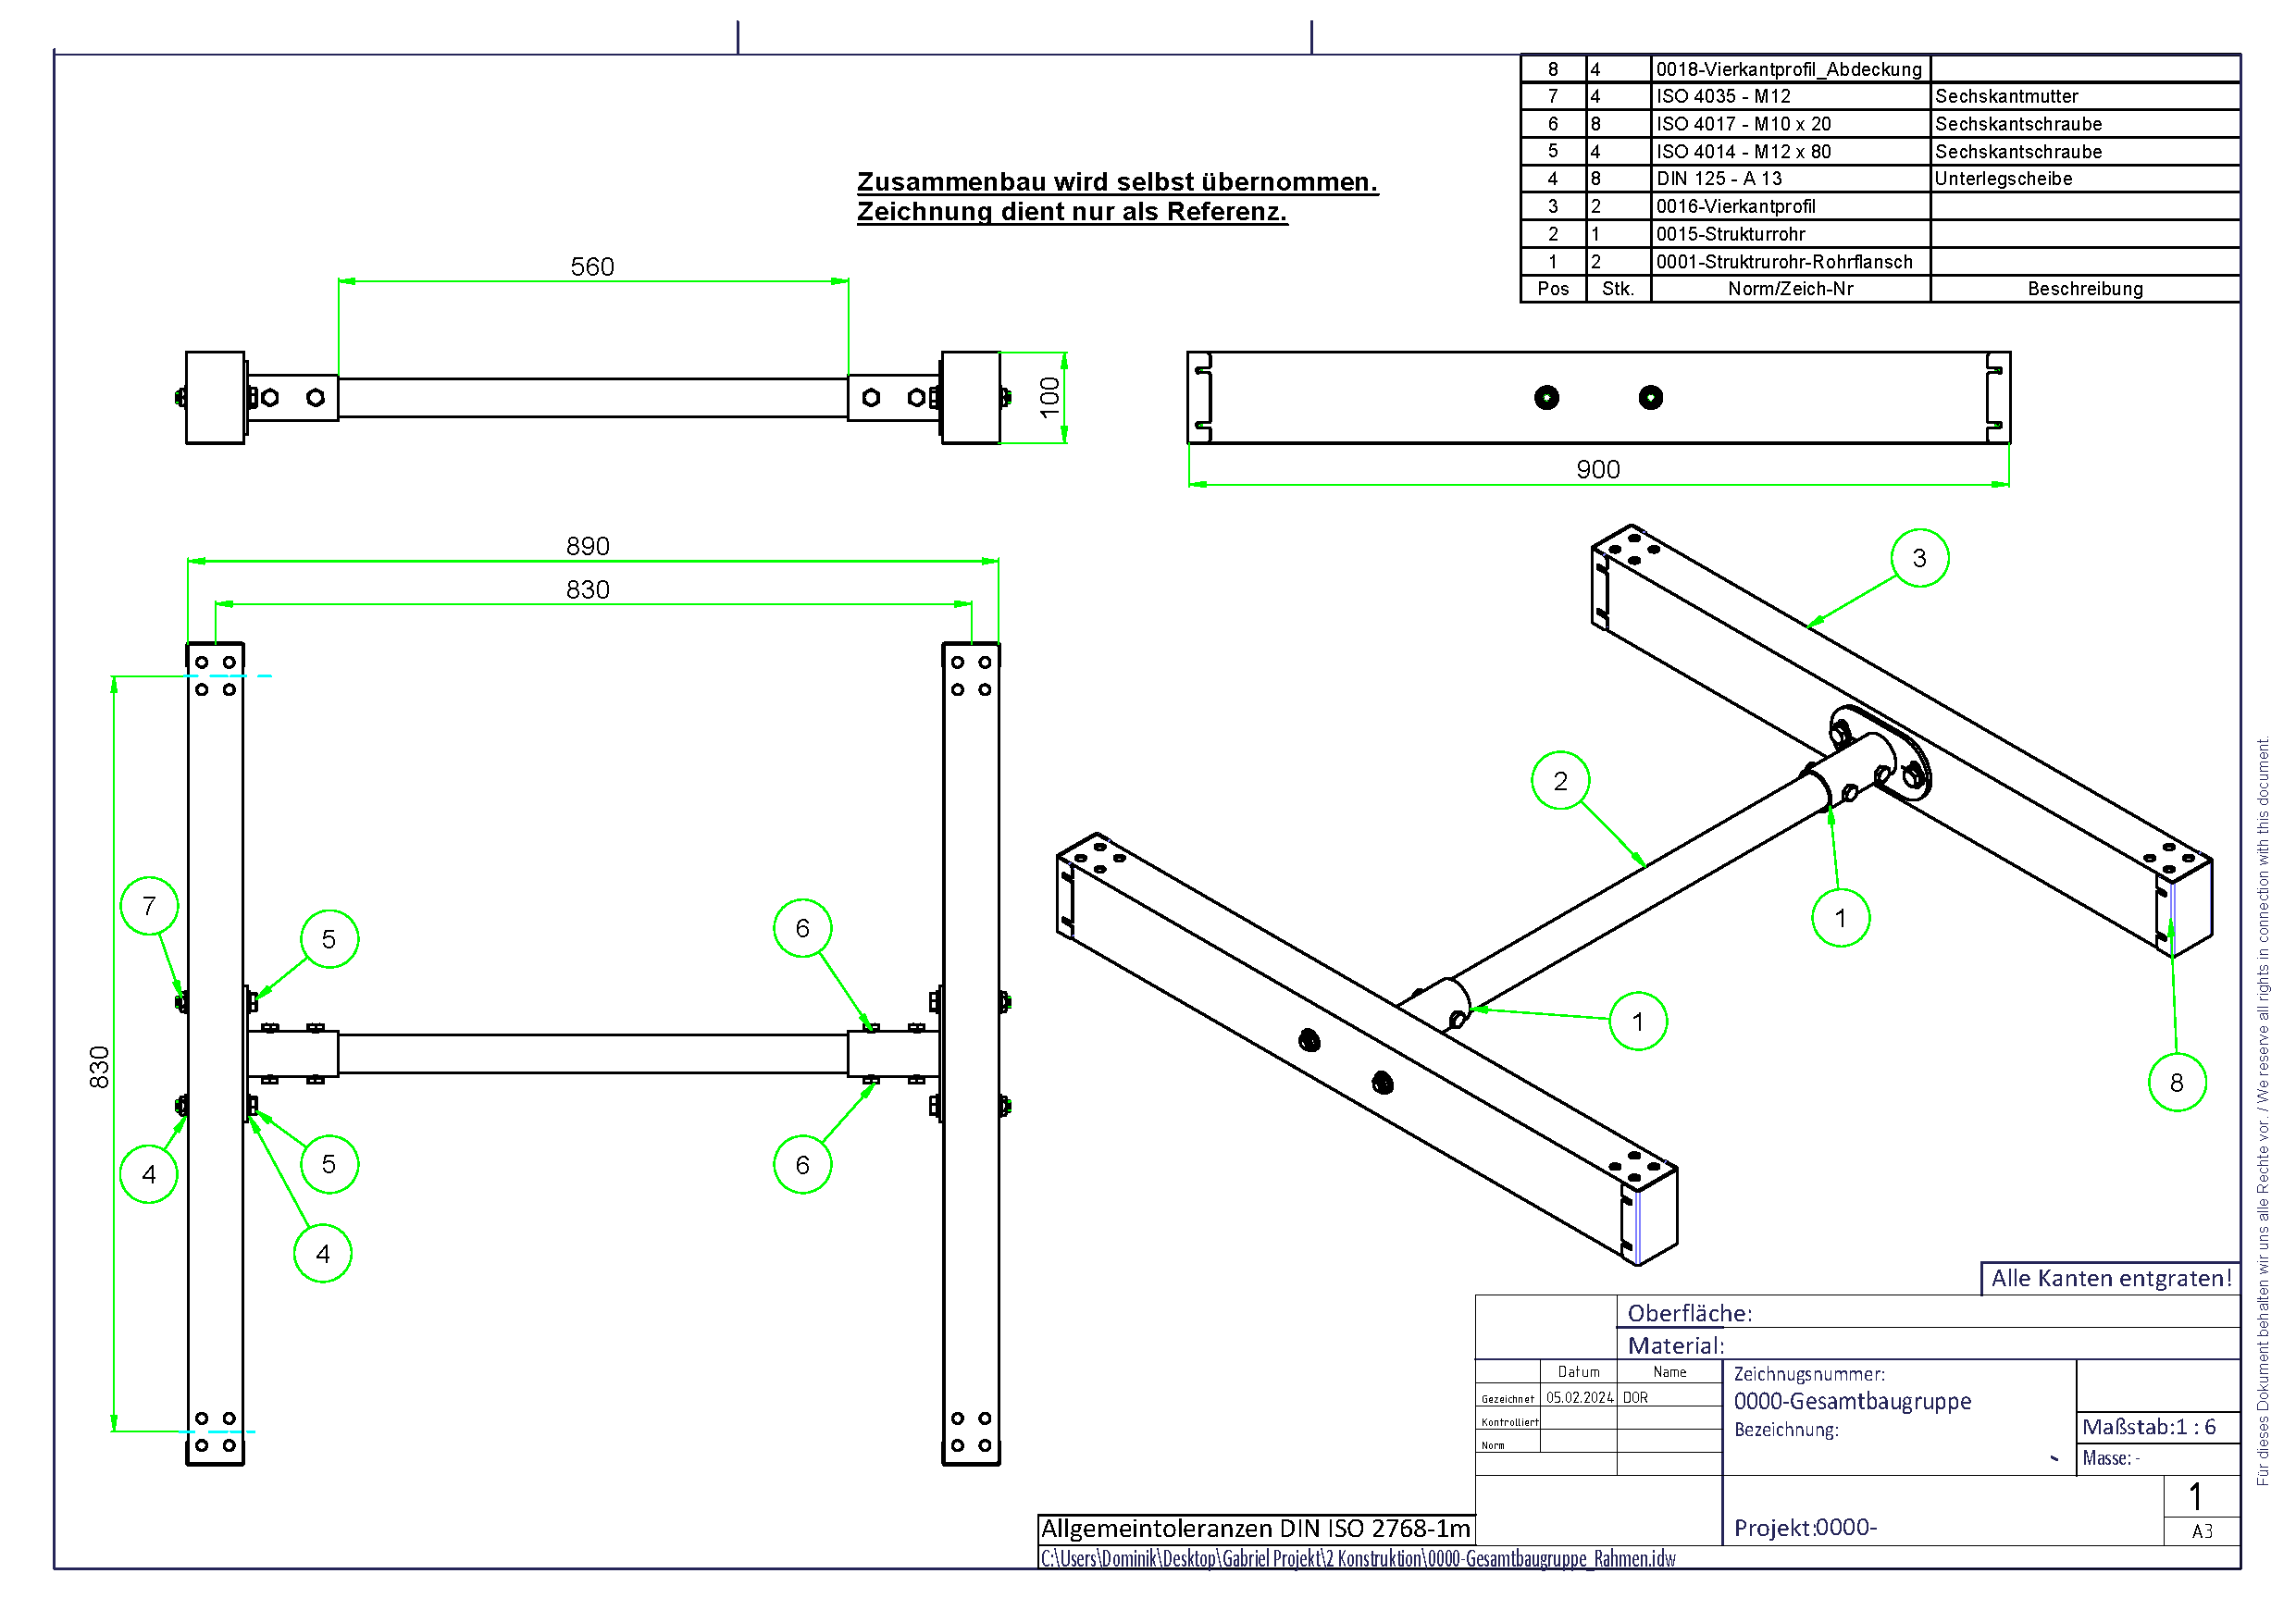
\includegraphics[keepaspectratio=true,scale=0.5]{../ref/0000-Gesamtbaugruppe_Rahmen.pdf}
	\caption{Bauplan des Gerüsts}
	\label{fig:Gerüst}
\end{figure}

Um eine komplette elektrische Isolierung der Antennen vom Gerüst zu ermöglichen, kommen Teflonplatten zum Einsatz. Diese verbinden die Antennen mit dem Aluminium-Vierkantprofil.

\begin{figure}[H]
	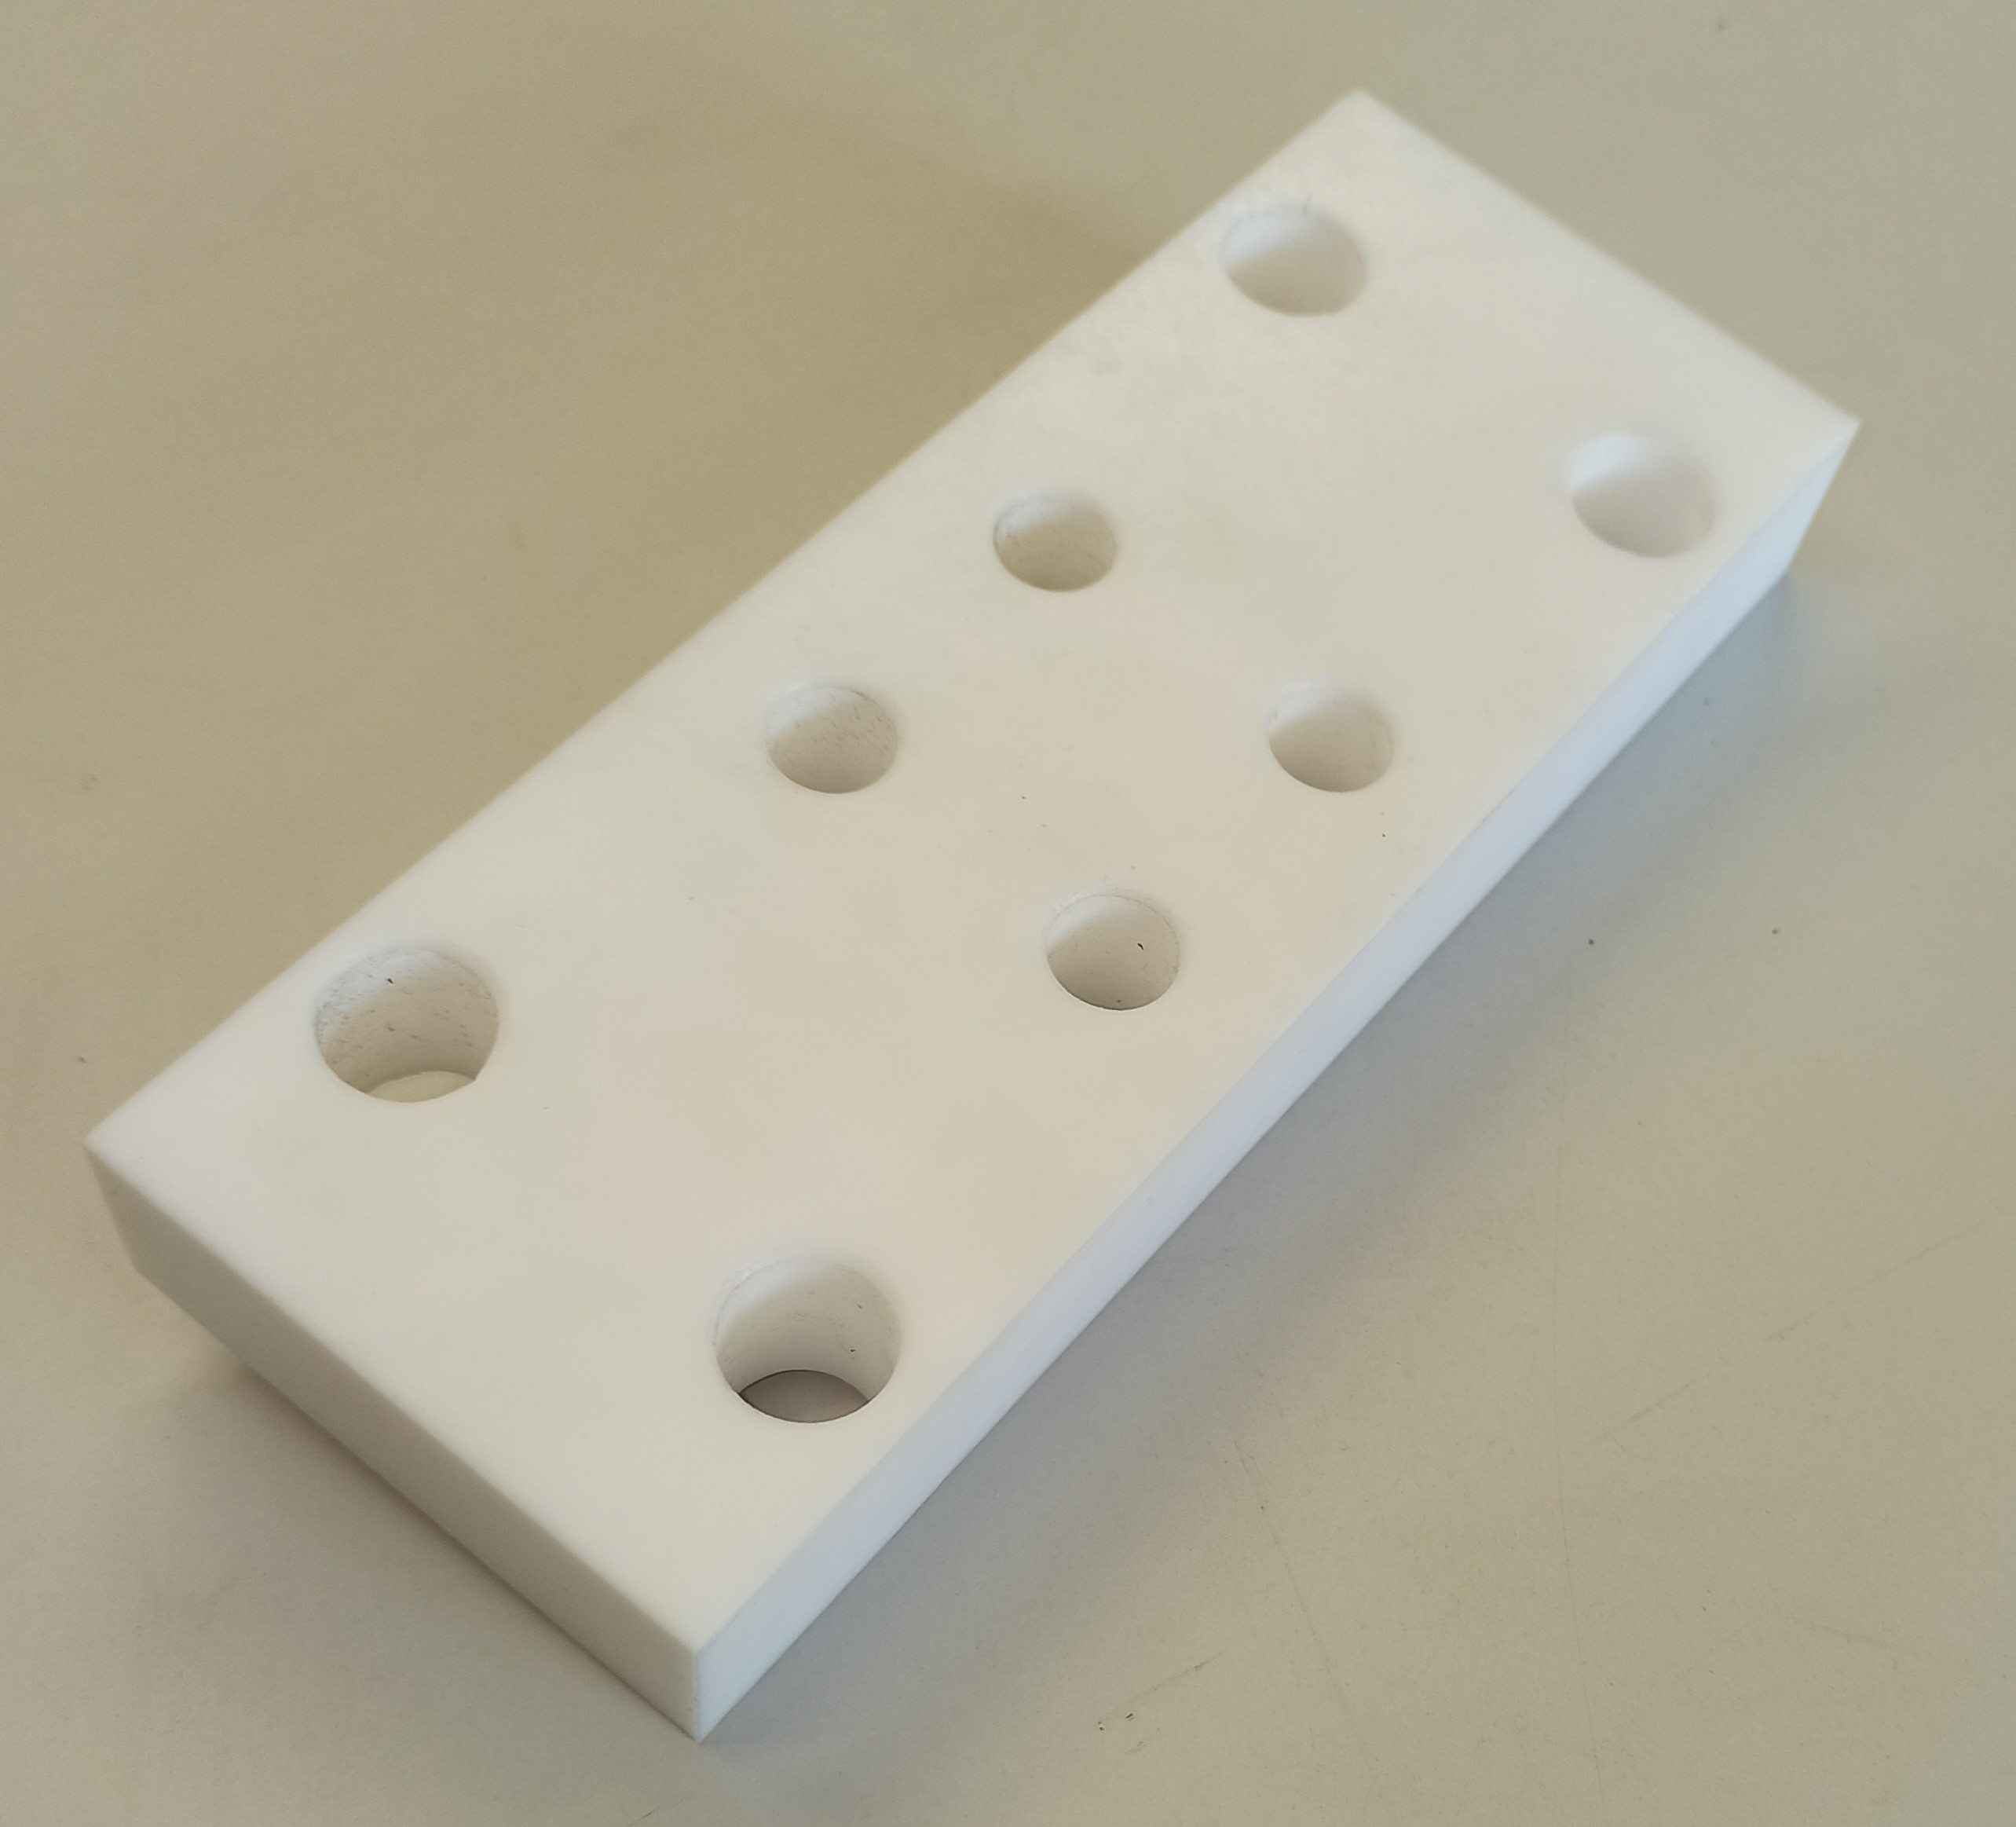
\includegraphics[width=\linewidth]{../ref/Teflon-Platte.jpg}
	\caption{Verbindende Teflonplatte}
	\label{fig:Teflonplatte}
\end{figure}

BILD DER VERBINDUNG

\subsection{Anpassung}
Da sich der Eingangswiderstand ändert, wenn vier solcher Antennen zusammen geschaltet werden, muss ein Anpassungsglied zwischen Koaxialkabel und Antennen eingesetzt werden. Hierbei wird eine Impedanz-Anpassungstechnik welche einfach zu implementieren ist. Diese besteht darin, einen Blechstreifen mit einer Länge von $\lambda/4$ an die erste Windung zu montieren. Dadurch wird die Impedanz auf 50$\Omega$ transformiert.

Der Anpassstreifen wurde mit zwei einzelnen Blechstreifen an dem unteren Ende der Helix angeschraubt.

BILD DER MONTAGE

Um nun vier Helixantennen zusammenzuschalten wird ein $\lambda/4$-Anpasstopf benötigt. Dieser verhält sich ähnlich wie ein Koaxialkabel, wobei das Verhältnis der Durchmesser zwischen Innenleiter und Außenleiter die Kapazität festlegt. Hierdurch kann der Wellenwiderstand angepasst werden.


BERECHNUNG

\cite{admin_lambda4_2016}

Es wurde hierbei die Variante mit einem viereckigen Außenleiter und einem runden Innenleiter angewendet, da sich die BNC-Buchsen an dem Vierkantrohr besser befestigen lassen.\\
Wird in die zuvor genannten Formeln eingesetzt, so erhält man die folgenden Ergebnisse.

BERECHNUNG



\subsection{Test}

Tests mit anderer Antenne im freien Feld